\chapter{Equazione di Schrodinger per Sistemi Unidimensionali}

	In questa sezione ci occupiamo del problema della determinazione degli autovalori dell'Hamiltoniana con un potenziale qualsiasi nel caso unidimensionale in vari casi. La particella è dunque vincolata a muoversi su una retta.
	
\section{Equazione di Schrodinger Unidimensionale}

\begin{nb}
	In generale l'operatore Hamiltoniano descrive l'energia di una particella che si muove in un potenziale (\textit{energia potenziale}) $V(x)$ tale che:
\begin{align*}
	\hat{H} = \frac{\hat{p}^2}{2m} + V(\hat{x})
\end{align*}
\end{nb}

	allora, data una funzione $\psi(x) \in L_2(\mathbb{R})$, il problema da risolvere, agli autovalori, è:
	
\begin{align*}
	\hat{H}\psi(x) = E \psi(x)
\end{align*}

	se scriviamo $\hat{H}$ in rappresentazione di Schrodinger si ha allora:

\begin{align*}
	& \hat{H}\psi(x) = E \psi(x) \\
	& \Leftrightarrow \, \qty[-\frac{\hbar^2}{2m} \dv[2]{x} + V(x) ] \psi(x) = E \psi(x) 
\end{align*}

	allora:
	
\begin{mydef}
	Si definisce \textbf{equazione di Schrodinger indipendente dal tempo ed unidimensionale} la seguente equazione:
\begin{align*}
	-\frac{\hbar^2}{2m} \dv[2]{x} \Psi(x) + V(x) \, \Psi(x) = E \, \Psi(x)
\end{align*}
\end{mydef}

	si tratta di \textit{una equazione differenziale del secondo ordine, lineare ed ordinaria}. Lo spazio delle soluzioni uno spazio vettoriale. Vediamo allora la generalizzazione a \textit{tre dimensioni:}
	
\begin{mydef}
	L'\textbf{equazione di Schrodinger tridimensionale} è:
\begin{align*}
	-\frac{\hbar^2}{2m} \nabla^{2} \Psi(\vb{r}) + V(\vb{r}) \, \Psi(\vb{r}) = E \, \Psi(\vb{r})
\end{align*}
\end{mydef}

	tornando ad una dimensione, fissato l'autovalore $E$, notiamo che lo spazio delle soluzione ha dimensione:
	
\begin{align*}
	\text{dim} \mathcal{H}_{E} = 2
\end{align*}

\begin{myapprf}
	Infatti anche se la particella si muove lungo una sola dimensione (l'asse $x$), l'equazione di Schrödinger in questo caso è un'equazione differenziale ordinaria del secondo ordine. Una equazione differenziale del secondo ordine ha, in generale, due soluzioni linearmente indipendenti. Ciò significa che qualsiasi soluzione $\Psi(x)$ si può scrivere come:

\begin{align*}
	\Psi(x) = c_1 \psi_1(x) + c_2 \psi_2(x)
\end{align*}

	dove $\psi_1(x),\psi_2(x)$ sono due soluzioni indipendenti e $c_1, c_2$ sono costanti arbitrarie determinate dalle condizioni iniziali o di bordo. Questo significa che, per un dato valore di energia $E$, la soluzione generale dell'equazione è una combinazione lineare di due soluzioni linearmente indipendenti.  Quindi, lo spazio delle soluzioni per un dato $E$ è bidimensionale (dimensione 2) perché abbiamo due gradi di libertà, ossia le due costanti $c_1, c_2$.
\end{myapprf}

	Vediamo ora due casi significativi e poi facciamo una discussione generale sulle caratteristiche che devono avere le soluzioni dell’equazione per essere fisicamente accettabili.

\subsection{Potenziale Armonico}

	Se ho un moto soggetto ad un potenziale armonico, ovvero del seguente tipo:
	
\begin{align*}
	V(x) = \frac{1}{2} \, m\omega^2 x^2
\end{align*}
	
	sostituendo nell'equazione di Schrodinger unidimensionale otteniamo:
	
\begin{align*}
	-\frac{\hbar^2}{2m} \dv[2]{x} \psi(x) + \textcolor{blue}{V(x)} \, \psi(x) = E \, \psi(x) \, \Rightarrow \, -\frac{\hbar^2}{2m}\psi''(x)  +\textcolor{blue}{\frac{1}{2} \, m\omega^2 x^2} \, \psi(x) =  E \, \psi(x)
\end{align*}

	la cui soluzione di fatto è già stata calcolata precedentemente. In questo caso conosciamo già gli autovalori $E_n$.

\subsection{Particella Libera}

	Nel caso della particella libera, si ha un potenziale nullo, ovvero:
	
\begin{align*}
	V(x) = 0
\end{align*}

	Allora in questo caso, l'Hamiltoniana è solo:

\begin{align*}
	\hat{H} = \frac{\hat{p}^2}{2m}
\end{align*}

	ovvero sia, che l'energia è solo cinetica. Poiché in questo modo vale che:
	
\begin{align*}
	\qty[\hat{H}, \hat{p}] = \hat{H}\hat{p} - \hat{p}\hat{H} = \qty(\frac{\hat{p}^2}{2m}) \, \hat{p} - \hat{p} \, \qty( \frac{\hat{p}^2}{2m} )  = \frac{1}{2m} \, \qty(\hat{p}^2\hat{p} - \hat{p}\hat{p}^2) = \frac{1}{2m} \, \qty(\hat{p}^3 - \hat{p}^3) = 0
\end{align*} 

	essendo che: $1/2m$ è una costante. Allora vale che, in questo caso della particella libera, l'Hamiltoniana commuta con l'operatore momento. Ciò cosa comporta?
	\\
	\\
	Se $\hat{H}$ ed $\hat{p}$ commutano allora essi hanno un insieme completo di autovettori (impropri) simultanei. Inoltre, poiché $\hat{p}$ è non degenere, allora ogni autovettore di $\hat{p}$ è anche autovettore di $\hat{H}$. Dunque i vettori $\ket{p}$ tali che
	
\begin{align*}
	\hat{p} \ket{p} = p \ket{p}
\end{align*}

	costituiscono una base di autovettori per $\hat{H}$ ed i corrispondenti autovalori $E$ si ottengono da:
	
\begin{align*}
	\hat{H} \ket{p} = E \ket{p} \, \Rightarrow \, \frac{p^2}{2m} \ket{p} = E \ket{p} \, \Rightarrow \, E = \frac{p^2}{2m} \geq 0
\end{align*}

	con il primo risultato importante ovvero che: l'energia è sempre positiva o nulla. Fissato dunque $E > 0$, l'equazione che segue:
	
\begin{align*}
	E = \frac{p^2}{2m} > 0
\end{align*}

	può essere risolta solo in due possibili modi per $p$, ovvero:

\begin{align*}
	p = + \sqrt{2mE} \qquad ; \qquad p = - \sqrt{2mE}
\end{align*}
	
	Questo implica che, fissata un'energia positiva $E$, abbiamo due autostati distinti che corrispondono allo stesso autovalore energetico:
	
\begin{align*}
	\ket{+p} \qquad ; \qquad \ket{-p} 
\end{align*}

	Il fatto che esistano due autostati distinti corrispondenti allo stesso autovalore $E$ implica che questo livello energetico è doppiamente degenere. Formalmente, ciò vuol dire che se un vettore $\ket{\psi}$ è autovettore di $\hat{H}$ con autovalore $E$, allora può essere espresso come combinazione lineare dei due autovettori degeneri:
	
\begin{align*}
	\ket{\psi} = \alpha \ket{+p} + \beta \ket{-p} \qquad \text{con : } \, \alpha, \beta \in \mathbb{C}
\end{align*}

	In altre parole, per ogni valore positivo fissato dell'energia, lo spazio degli autovettori associato (detto sottospazio degenere) ha dimensione $2$. Questa è proprio la definizione di degenerazione doppia. Inoltre è importante osservare che l'autovalore $E = 0$ è invece non degenere (o singolarmente degenere), dato che corrisponde a un unico valore di $p = 0$.
	\\
	\\
	Infine il significato fisico di questo risultato è che, poiché l’energia è solo cinetica, sia che la particella si muova da sinistra verso destra, sia che si muova da destra verso sinistra, purché con la stessa velocità, l’energia è la stessa. Si osservi la differenza tra la situazione classica e quella quantistica:
	
\begin{itemize}
	\item Classicamente, fissata l’energia $E$, sono possibili solo stati di moto in cui l’impulso è positivo o negativo.
	\item Quantisticamente, esistono stati di moto in cui la particella non ha una direzione di moto definita, ma viaggia contemporaneamente in due direzioni opposte.
\end{itemize}

\section{Operatore di Inversione Spaziale}

	Prima di procedere nello studio delle caratteristiche generali delle soluzioni dell'equazioni di Schrodinger, introduciamo due concetti particolarmente significativi. Il primo di questi concetti è un \textit{teorema estremamente importante}:

\subsection{Teorema di Degenerazione}
	
\begin{myth}
	Se due osservabili $\alpha$ e $\beta$ commutano entrambe con un'osservabile $\gamma$, ma non commutano tra di loro, ovvero:
\begin{align*}
	\qty\Big[\hat{\gamma}, \hat{\alpha}] = 0 \quad ; \quad \qty[\hat{\gamma}, \hat{\beta}] = 0 \quad ; \quad \qty[\hat{\alpha}, \hat{\beta}] \neq 0 \quad ; \quad 
\end{align*}
	allora vale che: $\gamma$ è \textbf{degenere}.
\end{myth}

\begin{myprf}
	La dimostrazione è immediata. Infatti se $\gamma$ non fosse degenere ogni suo autovettore sarebbe anche autovettore di $\alpha$ e $\beta$, e quindi ne seguirebbe che $\alpha$ e $\beta$ avrebbero un insieme completo di autovettori simultanei e perciò commuterebbero, contraddicendo l'ipotesi di partenza.
\end{myprf}

	Il secondo concetto invece è proprio l'introduzione del seguente operatore:

\subsection{Operatore di Inversione Spaziale}

	Introduciamo il concetto di \textbf{operatore di inversione spaziale} nel seguente modo:
	
\begin{mydef}
	Definiamo l'\textbf{operatore di inversione spaziale} $\hat{I}$ come:
\begin{align*}
	\hat{I} : \psi(x) \to \psi(-x)
\end{align*}
	tale che:
\begin{align*}
	\hat{I}\psi(x) = \psi(-x)
\end{align*}
\end{mydef}

	per quanto riguarda gli operatori $\hat{x}$ ed $\hat{p}$ siccome le seguenti trasformazioni:
	
\begin{align*}
	\hat{x} \to -\hat{x} \quad ; \quad \hat{p} \to -\hat{p}
\end{align*}

	sono canoniche (si ricorda che per trasformazione canonica si intende una trasformazione che mantiene la forma delle parentesi di Poisson e perciò una trasformazione canonica è, in sostanza, una trasformazione che preserva la struttura fondamentale dello spazio delle fasi e che non altera la forma canonica delle equazioni di Hamilton). Allora $\hat{I}$ è l'operatore unitario che ne inverte i segni per coniugazione, cioè:

\begin{nb}	
	$\hat{I}$ è tale che:
\begin{align*}
	& \hat{I} : \hat{x} \to - \hat{x} \quad \text{tale che} \quad \hat{I}^{-1}\hat{x}\hat{I} = - \hat{x} \\
	& \hat{I} : \hat{p} \to - \hat{p} \quad \text{tale che} \quad \hat{I}^{-1}\hat{p}\hat{I} = - \hat{p} 
\end{align*} 
\end{nb}

	Perché ci interessa questo nuovo operatore? 
	\\
	\\
	Capiamo come agisce su $\hat{H}$, noi sappiamo che:
	
\begin{align*}
	\hat{H} = \frac{\hat{p}^2}{2m} + V(\hat{x})
\end{align*}

	allora:
	
\begin{align*}
	\hat{I}^{-1}\hat{H}\hat{I} = \hat{I}^{-1}\frac{\hat{p}^2}{2m}\hat{I} + \hat{I}^{-1}V(\hat{x})\hat{I} = \frac{1}{2m} \, \textcolor{orange}{\hat{I}^{-1}\hat{p}^2\hat{I}} + \textcolor{blue}{\hat{I}^{-1}V(\hat{x})\hat{I}} &= \frac{1}{2m} \, \textcolor{orange}{\hat{I}^{-1}\hat{p}\hat{I} \, \hat{I}^{-1}\hat{p}\hat{I}} + \textcolor{blue}{V(-\hat{x})} \\
	& =  \frac{1}{2m} \, \textcolor{orange}{\hat{p}^2} +V(-\hat{x}) \\
	& =  \frac{\hat{p}^2}{2m} +V(-\hat{x}) 
\end{align*}
	
	In particolare, se il potenziale è \textit{simmetrico}, cioè se:
	
\begin{align*}
	V(\hat{x}) = V(-\hat{x})
\end{align*}

	si ha che:
	
\begin{align*}
	 \hat{I}^{-1}\hat{H}\hat{I}= \hat{H} \, \Rightarrow \, \hat{H}\hat{I} = \hat{I}\hat{H} \, \Rightarrow \, \qty[\hat{H}, \hat{I}] = 0
\end{align*}
	
	ossia abbiamo che $\hat{I}$ ed $\hat{H}$ commutano. In generale, come vedremo più avanti, operatori che commutano con $\hat{H}$ \textit{corrispondono a simmetrie}.

\subsection{Proprietà dell'Operatore di Inversione Spaziale}

\begin{nb}
	Valgono le seguenti generiche \textit{proprietà:}
\begin{enumerate}[label=\arabic*)]
	\item $\hat{I}^2 = \mathbb{I}$ 
	\item $\hat{I} = \hat{I}^{\dagger}$
	\item $\hat{I}^{\dagger} = \hat{I}^{-1}$
\end{enumerate}
\end{nb}

	Sia $\psi(x)$ un'autofunzione di $\hat{I}$ corrispondente all'autovalore $\lambda$, ovvero tale che:
	
\begin{align*}
	\textcolor{cyan}{\hat{I}\psi(x)} = \lambda \psi(x)
\end{align*}

	applico allora $\hat{I}$ ad ambo i membri ovvero:

\begin{align*}
	\hat{I}^2\psi(x) = \lambda \, \textcolor{cyan}{\hat{I}\psi(x)} \, \Rightarrow \, \psi(x) = \lambda^2 \, \psi(x)
\end{align*}

	quindi ho subito che:
	
\begin{align*}
	\lambda^2 = 1
\end{align*}

	ossia: $\lambda = \pm 1$. Pertanto le autofunzioni di $\hat{I}$ sono quelle tali che:
	
\begin{align*}
	\hat{I} \psi(x) = \pm \, \psi(x) \, \Rightarrow \, \psi(-x) = \pm \psi(x)
\end{align*}
	
	dunque:
	
\begin{itemize}
	\item Per $\lambda = +1 \, \Rightarrow$ ho autovettori \textbf{pari} rispetto all'inversione $x \to -x$, cioè $\psi(x) = \psi(-x)$.
	\item Per $\lambda = -1 \, \Rightarrow$ ho autovettori \textbf{dispari} rispetto all'inversione $x \to -x$, cioè $\psi(x) = - \psi(-x)$.
\end{itemize}

	dunque vale che $\lambda$ ci da la parità dell'autovettore.

\section{Caratteristiche Generali delle Soluzioni dell’Equazione di
Schrodinger nel Caso Unidimensionale}

	L'obiettivo ora è quello di studiare le caratteristiche generali che devono avere le soluzioni dell'equazione di Schrodinger in una dimensione affinché siano fisicamente accettabili. Ci interessano quindi le caratteristiche generali degli autovalori e delle autofunzioni dell'Hamiltoniana di una particella soggetta a muoversi su una retta in un potenziale $V(x)$. Come già detto, ci interessano soltanto quelle soluzioni $\psi(x)$ del tipo:
	
\begin{enumerate}[label=\arabic*)]
	\item $\psi(x) \in L_2(\mathbb{R})$ che tendono a zero per $x \to \pm \infty$ 
		
		Queste sono autofunzioni proprie di $\hat{H}$ e corrispondono agli stati legati del sistema: la probabilità di trovare la particella per $|x| > L$ tende a zero per $L \to \infty$. I corrispondenti autovalori sono propri, cioè livelli energetici discreti del sistema.
		
	\item $\psi(x) \notin L_2(\mathbb{R})$ che si mantengono limitate per $x \to \pm \infty$
	
		Queste sono le autofunzioni improprie di $\hat{H}$ ed i corrispondenti autovalori sono impropri e formano uno spettro continuo.
\end{enumerate}

	Notiamo che possiamo limitarci a considerare soltanto soluzioni reali dell'equazione, infatti qualunque sia il valore di $E$ (purché reale, dato che abbiamo trovato che gli autovalori di $\hat{H}$ sono reali), se $\psi(x)$ è una soluzione anche $\psi^*(x)$ lo è, perché l'equazione differenziale è a coefficienti reali.
	\\
	\\
	Sia $V(x)$ arbitrario e si fissi un valore di $E$ qualunque: in questo modo l'asse delle $x$ è suddiviso in regioni di due tipi:
	
\begin{itemize}
	\item Regioni di tipo $1 \, \Rightarrow \, $ classicamente permesse $\, \Rightarrow \, $ regioni in cui $E \geq V(x)$
	\item Regioni di tipo $2 \, \Rightarrow \, $ classicamente proibite $\, \Rightarrow \, $ regioni in cui $E < V(x)$
\end{itemize}

%%%%%%%
\vspace{1em}
%%%%%%%
\begin{center}
\begin{tikzpicture}[scale=1.1]
    % Assi
    \draw[->] (-5,0) -- (5,0) node[right] {$x$};
    \draw[->] (0,-0.5) -- (0,4) node[above] {$V(x)$};

    % Funzione potenziale generica (alzata di 0.5)
    \draw[thick, domain=-4.5:4.5, smooth, variable=\x, blue]
        plot ({\x}, {1.3*sin(deg(\x))+1.5+0.05*\x^2});

    % Linea rossa ai punti critici x_c (alzata)
    \draw[red, thick] (-5,2) -- (5,2) node[right] {$E$};
    
     \draw[dashed, thick] (0.4, 0) -- (0.4,2);
      \draw[dashed, thick] (3.1, 0) -- (3.1,2);

    % Etichette sezioni aggiornate (Regione 1 sopra, Regione 2 sotto linea rossa)
    \node at (-2,1) {1};
    \node at (4,1) {1};
    \node at (1.7,1) {2};

\end{tikzpicture}
\end{center}
%%%%%%%
\vspace{1em}
%%%%%%%

	I punti di confine tra le due regioni, cioè tali che $E = V(x)$, sono detti \textbf{punti di inversione} del moto. Dal punto di vista dell'equazione di Schrodinger si ha che:
	
\begin{align*}
	- \frac{\hbar^2}{2m} \, \psi''(x) + V(x) \psi(x) = E \psi(x) 
\end{align*}

	o anche:
	
\begin{align*}
	\psi''(x) = \frac{2m}{\hbar} \, \qty\Big(V(x) - E ) \, \psi(x)
\end{align*}

	pertanto:
	
\begin{enumerate}[label=\arabic*)]
	\item Nelle regioni di tipo $1$, ovvero dove:
	\begin{align*}
		V(x) - E < 0
	\end{align*}
		
%%%%%%%
\vspace{1em}
%%%%%%%
\begin{minipage}{0.5\textwidth}
\begin{tikzpicture}[scale=0.6]
    % Assi
    \draw[->] (-5,0) -- (5,0) node[right] {$x$};
    \draw[->] (0,-5) -- (0,5) node[above] {$\psi(x)$};
    
     % Prima parabola concava (sinistra, primo quadrante)
    \draw[thick, domain=-5:-1.5, smooth, variable=\x, blue]
        plot ({\x}, {-0.5*(\x+3)^2+4});

    % Seconda parabola convessa (destra, terzo quadrante)
    \draw[thick, domain=1.5:5, smooth, variable=\x, red]
        plot ({\x}, {0.5*(\x-3)^2-4});
    
	%%%
    
     \draw[dashed, thick] (-3,4) -- (-3, 0) node[below] {$x$};
      \draw[dashed, thick] (3, -4)-- (3, 0) node[above] {$x$};

\end{tikzpicture}
\end{minipage}
\hfill
\begin{minipage}{0.5\textwidth}

	vale allora che:
\begin{align*}
	\frac{\psi''(x)}{\psi(x)} < 0
\end{align*}
	da cui deduco che la concavità è diretta verso l'asse delle $x$ e che $\psi_E(x)$ è oscillante.
	
\end{minipage}
%%%%%%%
\vspace{1em}
%%%%%%%
	
	\item Nella regioni di tipo 2 invece dove:
	\begin{align*}
		V(x) - E > 0
	\end{align*}
		e quindi vale:
		
%%%%%%%
\vspace{1em}
%%%%%%%
\begin{minipage}{0.5\textwidth}
\begin{tikzpicture}[scale=0.6]
    % Assi
    \draw[->] (-5,0) -- (5,0) node[right] {$x$};
    \draw[->] (0,-5) -- (0,5) node[above] {$\psi(x)$};
    
     \draw[->] (-5,0) -- (5,0) node[right] {$x$};
    \draw[->] (0,-5) -- (0,5) node[above] {$\psi(x)$};

    % Parabola convessa sopra nel I quadrante (alto-destra)
    \draw[thick, domain=1.2:4, smooth, variable=\x, blue]
        plot ({\x}, {0.6*(\x - 2.6)^2 + 1});

    % Parabola convessa sopra nel II quadrante (alto-sinistra)
    \draw[thick, domain=-4:-1.2, smooth, variable=\x, blue]
        plot ({\x}, {0.6*(\x + 2.6)^2 + 1});

    % Parabola concava sotto nel III quadrante (basso-sinistra)
    \draw[thick, domain=-4:-1.2, smooth, variable=\x, blue]
        plot ({\x}, {-0.6*(\x + 2.6)^2 - 1});

    % Parabola concava sotto nel IV quadrante (basso-destra)
    \draw[thick, domain=1.2:4, smooth, variable=\x, blue]
        plot ({\x}, {-0.6*(\x - 2.6)^2 - 1});
\end{tikzpicture}
\end{minipage}
\hfill
\begin{minipage}{0.5\textwidth}

\begin{align*}
	\frac{\psi''(x)}{\psi(x)} > 0
\end{align*}
	da cui deduco che la concavità è diretta in maniera opposta rispetto all'asse delle $x$ e che $\psi_E(x)$ tende ad "allontanarsi" dall'asse delle $x$.
\end{minipage}
%%%%%%%
\vspace{1em}
%%%%%%%
	
\end{enumerate}

	Per capire se una soluzione è accettabile o no, studiamo i comportamenti a $x \to \pm \infty$ nei seguenti casi:

\begin{itemize}
	\item Le regioni $x \to \pm \infty$ sono entrambe di tipo $1 \, \Rightarrow \, (1, 1)$.
	\item Le regioni $x \to \pm \infty$ sono entrambe di tipo $2 \, \Rightarrow \, (2, 2)$.
	\item Le regioni $x \to \pm \infty$ sono una di tipo $1$ ed una di tipo $2 \, \Rightarrow \, (1, 2)$ o $(2, 1)$.
\end{itemize}
	
	tuttavia questi non sono tutti i casi possibili. Vi sono casi in cui per $x \to \pm \infty$ vi è un'alternanza infinita di regioni di tipo $1$ e di tipo $2$. Questo succede, ad esempio, con i potenziali periodici, per i quali lo spettro è discreto e a \textbf{bande}. Dunque fissata $E$, analizziamo i tre casi appena elencati:

\begin{enumerate}[label=\arabic*)]

	\item In questo caso la soluzione ha un comportamento oscillante e, se il potenziale è limitato:
	%%%%%%%
	\vspace{1em}
	%%%%%%%
	
	\begin{minipage}{0.5\textwidth}
	\begin{tikzpicture}[scale=0.6]
    		% Assi
    		\draw[->] (-5,0) -- (5,0) node[right] {$x$};
    		\draw[->] (0,-5) -- (0,5) node[above] {$\psi(x)$};
    
    	 	\draw[->] (-5,0) -- (5,0) node[right] {$x$};
    		\draw[->] (0,-5) -- (0,5) node[above] {$\psi(x)$};
		
	% Linee verticali a x=-2 e x=2
    	\draw[thick,dashed] (-2,-5) -- (-2,5);
    	\draw[thick,dashed] (2,-5) -- (2,5);
	
	% regioni
	\node at (-4, -4) {$1$}; 
	\node at (4, -4) {$1$};
	
	% tangente e punto x_0
	\filldraw (-4.62, 3) circle (2pt);
	\draw [dashed] (-4.62, 3) -- (-4.62, 0) node [below] {$x_0$};
	\draw [thick, dashed, red] (-6,2) -- (-3,4);

	 % Sinusoide corretta a sinistra con deg()
    \draw[thick,domain=-5:-2, smooth, variable=\x, ForestGreen]
        plot ({\x},{3*sin(deg(2*pi*(\x+5)/1.5))});

    % Sinusoide modificata a destra
    \draw[thick,domain=2:5,smooth,variable=\x, ForestGreen]
        plot ({\x},{-3*cos(deg(1.5*(\x-2))) - 0.4*(\x-2)^2 +5});

    	% Zona centrale con righe oblique blu
    	\fill[pattern=north east lines, pattern color=blue!60] 
        (-2,-5) rectangle (2,5);
        
	\end{tikzpicture}
	\end{minipage}
	\hfill
	\begin{minipage}{0.5\textwidth}
		allora la soluzione si manterrà limitata per $|x| \to \infty$ per ogni valore di $E$ e qualunque sia la condizione iniziale del problema di Cauchy sulla pendenza in un punto qualsiasi $\psi'(x_0)$. Pertanto in questo caso l'energia ha spettro continuo con degenerazione $2$: cioè ho due parametri liberi, $E$ e $\psi'(x_0)$. In questo caso non conosco il comportamento di $\psi(x)$ in centro.
	\end{minipage}
	%%%%%%%
	\vspace{1em}
	%%%%%%%
	
	\item In questo caso, per concavità, se tutta la retta reale $x$ è di tipo $2$, la funzione d'onda diverse sia per $x \to - \infty$ che per $x \to + \infty$. In tal caso non ho soluzioni accettabili in nessun caso. Se invece $E$ è maggiore del valore minimo di $V(x)$ allora vi è almeno una regione di tipo $1$ tra le due regioni asintotiche di tipo $2$. In queste ultime, la funzione d'onda rimane limitata solo se tende a zero.
	%%%%%%%
	\vspace{1em}
	%%%%%%%
	
	\begin{minipage}{0.5\textwidth}
	\begin{tikzpicture}[scale=0.6]
    		% Assi
    		\draw[->] (-6.5,0) -- (6.5,0) node[right] {$x$};
    		\draw[->] (0,-5) -- (0,5) node[above] {$\psi(x)$};
		
	% Linee verticali a x=-2 e x=2
    	\draw[thick,dashed] (-2,-5) -- (-2,5);
    	\draw[thick,dashed] (2,-5) -- (2,5);
	
	% regioni
	\node at (-4, -4) {$2$}; 
	\node at (4, -4) {$2$};
	\node at (0, -6) {$1$};

    	% Zona centrale con righe oblique blu
    	\fill[pattern=north east lines, pattern color=blue!60] 
        (-2,-5) rectangle (2,5);
        
        \draw[thick,domain=-6.5:-2,smooth,samples=100,variable=\x, ForestGreen]
         plot ({\x},{4*exp(-ln(4/3)*((-\x-3)^2))});
       \draw[thick,domain=2:6.5,smooth,samples=100,variable=\x, ForestGreen]
         plot ({\x},{-4*exp(-ln(4/3)*((\x-3)^2))});
        
	\end{tikzpicture}
	\end{minipage}
	\hfill
	\begin{minipage}{0.35\textwidth}
		Per ogni valore di $E$ posso, ad esempio, modificare $\psi'(x_0)$ in modo tale che $\psi(x)$ vada a zero per infinito, ad esempio per $x \to -\infty$. Per valori generici di $E$, in genere, fissato $\psi'(x_0)$ ad $x \to + \infty$ la soluzione diverge. Ho quindi esaurito le "scelte": soltanto per particolari valori di $E$ accade che la soluzione converge a zero sia a destra che a sinistra, pertanto in questo caso ho uno spettro discreto con degenerazione $1$: ho valori fissi di $E$, posso variare solo $\psi'(x_0)$.
	\end{minipage}
	%%%%%%%
	\vspace{1em}
	%%%%%%%

	\item In questo ultimo caso, per $(1, 2)$ tanto quanto per $(2, 1)$, per ogni valore di $E$ possiamo modificare $\psi'(x_0)$ in modo tale che:
	%%%%%%%
	\vspace{1em}
	%%%%%%%
	
	\begin{minipage}{0.5\textwidth}
	\begin{tikzpicture}[scale=0.6]
    		% Assi
    	\draw[->] (-5,0) -- (6.5,0) node[right] {$x$};
    	\draw[->] (0,-5) -- (0,5) node[above] {$\psi(x)$};
		
	% Linee verticali a x=-2 e x=2
    	\draw[thick,dashed] (-2,-5) -- (-2,5);
    	\draw[thick,dashed] (2,-5) -- (2,5);
	
	% regioni
	\node at (-4, -4) {$1$}; 
	\node at (4, -4) {$2$};

\draw[thick,domain=-5:-2,smooth,variable=\x, ForestGreen]
        plot ({\x},{3*sin(deg(2*pi*(\x+5)/1.5))});

    	% Zona centrale con righe oblique blu
    	\fill[pattern=north east lines, pattern color=blue!60] 
        (-2,-5) rectangle (2,5);
        
        % Funzione a destra: definita per x in [2,5]
    % Utilizziamo una forma gaussiana modificata:
    %    ψ(x)= 4 exp[-ln(4/3)·(x-3)^2],
    % che garantisce ψ(2)=3, ψ(3)=4, e decrescenza per x>3
    \draw[thick,domain=2:6.5,smooth,samples=100,variable=\x, ForestGreen]
         plot ({\x},{4*exp(-ln(4/3)*((\x-3)^2))});

	\end{tikzpicture}
	\end{minipage}
	\hfill
	\begin{minipage}{0.4\textwidth}
		la soluzione nella regione di tipo $2$ non diverga, mentre nella regione di tipo $1$ avrò un comportamento oscillatorio. Pertanto $E$ ha uno spettro continuo con degenerazione $1$: fissato $\psi'(x_0)$ posso variare $E$.
	\end{minipage}
	%%%%%%%
	\vspace{1em}
	%%%%%%%
\end{enumerate}

\section{Sistemi Unidimensionali}

	Vedremo ora diversi esempi di sistemi unidimensionali soggetti a diversi tipi di potenziale. In molte situazioni fisiche si ha a che fare con potenziali $V(x)$ che in un intervallo molto piccolo (scegliamo di ampiezza $2\varepsilon$) passano da un valore $V_1$ ad un altro valore $V_2$:

%%%%%%%
\vspace{1em}
%%%%%%%
	
\begin{minipage}{0.4\textwidth}
	Ad esempio, un elettrone vicino alla superficie di un metallo è soggetto ad un potenziale che in un intervallo di pochi Å passa dal valore che ha dentro il metallo al valore che assume fuori. In situazioni del genere, sia per la scarsa conoscenza di $V(x)$, sia per comodità, si è soliti sostituire ad un potenziale di questo tipo, o meglio approssimarlo, un potenziale continuo a tratti, prendendo il limite per $\varepsilon \to 0$. Si consideri dunque l’equazione di Schrodinger e si integrino ambo i membri nell’intervallo $2\varepsilon$ centrato in $x = 0$:
\begin{align*}
	- \frac{\hbar^2}{2m} \int_{-\varepsilon}^{\, + \varepsilon} \psi''(x) \, \dd x = \int_{-\varepsilon}^{\, + \varepsilon} \qty\Big[E - V(x)] \,  \psi(x) \, \dd x 
\end{align*}
\end{minipage}
	\hfill
\begin{minipage}{0.5\textwidth}

\begin{tikzpicture}[scale=0.6]
	% Assi
    		\draw[->] (-5,0) -- (7.5,0) node[right] {$x$};
    		\draw[->] (0,-5) -- (0,6.5) node[above] {$V(x)$};
		
	% Linee verticali a x=-2 e x=2
    	\draw[thick,dashed] (-2,-5) -- (-2,6.5);
    	\draw[thick,dashed] (2,-5) -- (2,6.5);
	
	% V0
	\draw[<->, thick, cyan, dashed] (6.5, 6) -- (6.5,0) node [midway, right] {$V_0$};
	
	\node at (-2.5, -0.5) {$-\varepsilon$}; 
	\node at (2.5, -0.5) {$+\varepsilon$};
	
	% funzioni
	
	\draw[thick, domain= -5: 0, smooth, samples=100,variable=\x, ForestGreen]
         plot ({\x},{3.5*exp(\x)});
         
        % Parte di raccordo: funzione monotona per x in [0,5]
  \draw[thick, domain=0:5, smooth, samples=100, variable=\x, ForestGreen]
       plot ({\x},{6 - 2.5*(1-\x/5)^7});

  % Parte destra: tratto costante pari a V_0 (qui 6) per x>=5
  \draw[thick, ForestGreen] (5,6) -- (7,6);
	
\end{tikzpicture}

\end{minipage}
%%%%%%%
\vspace{1em}
%%%%%%%

	Poiché il potenziale rimane limitato nella regione: $\qty[- \varepsilon, + \varepsilon]$ ed in $x = 0$, si ha che:
	
\begin{align*}
	- \frac{\hbar^2}{2m} \, \qty\Big[\psi'(\varepsilon) - \psi'(-\varepsilon)] \simeq 2\varepsilon \, \qty\Big[E - V(0)] \, \psi(0) + \order{4\varepsilon^2}
\end{align*}

	dunque per $\varepsilon \to 0^+$, concludiamo che:
	
\begin{align*}
	\lim_{\varepsilon \to 0^+} \qty\Big[\psi'(\varepsilon) - \psi'(- \varepsilon)] = 0
\end{align*}

	Ciò significa che la derivata prima della funzione d'onda è continua $x = 0$, cioè a maggior ragione, che la funzione d'onda stessa è continua in $x = 0$ e in particolare, sotto queste condizioni, in ogni discontinuità.

\subsection{Gradino di Potenziale}

	Si consideri una particella in moto sull'asse reale soggetta al potenziale che segue:
	
\begin{align*}
	V(x) = \begin{cases}
		0 \quad \text{se} \quad x < 0 \\
		V_0  \quad \text{se}  \quad x > 0
	\end{cases}
\end{align*}

	dove $V_0 > 0$.
	\\
	\\
 	Le traiettorie classiche sono di due tipi, quelle per cui vale:
\begin{enumerate}[label=\arabic*)]

	\item $0 < E < V_0$
		
		Le quali sono confinate in $x < 0$, esse corrispondono a particelle provenienti da $x = -\infty$ che rimbalzano sul gradino $x = 0$ e viaggiano indietro $x \to \infty - \infty$ con la stessa energia cinetica ed impulso opposto. 
		
	\item $E > V_0$
	
		Queste traiettorie invece corrispondono sia a particelle provenienti da $x \to - \infty$ con impulso pari a:
	\begin{align*}
		p = \sqrt{2mE}
	\end{align*}
		e che viaggiano verso $x \to +\infty$ con impulso ridotto:
	\begin{align*}
		p' = \sqrt{2m\qty(E - V_0)}
	\end{align*}
		sia a particelle con la traiettoria opposta, provenienti da $x \to +\infty$ con impulso $- p'$ e viaggianti verso $x \to -\infty$ con impulso $-p$. 
\end{enumerate}

	Dai discorsi precedenti sappiamo che lo spettro di $E$ deve essere positivo. Vediamo cosa succede alle soluzione al variare di $E$, in un contesto quantistico:

%%%%%%%
\vspace{1em}
%%%%%%%
\begin{center}
\begin{tikzpicture}[scale=0.8]
	% Assi
    	\draw[->] (-5, 0) -- (5, 0) node[right] {$x$};
    	\draw[->] (0, -2) -- (0, 5) node[above] {$V(x)$};
	
	
	% funzione
	\draw[ thick, red] (-4, 0) -- (0, 0);
	\draw[ thick, red] (0, 0) -- (0, 4);
	\draw[ thick, red] (0, 4) -- (4, 4);
	
\end{tikzpicture}
\end{center}
%%%%%%%
\vspace{1em}
%%%%%%%

\begin{enumerate}[label=\arabic*)]

	\item \textbf{Riflessione totale:} $0 < E < V_0$
	
		In questo caso $p'$ è puramente immaginario, ovvero sia tale che:
	\begin{align*}
		p' = i \, |p'| = i \, \sqrt{2m \, \qty(V_0 - E)}
	\end{align*}
	
		siano allora:
		
	\begin{align*}
		k \, \equiv \, \frac{p}{\hbar} \quad ; \quad k' \, \equiv \, \frac{p'}{\hbar}
	\end{align*}
	
	allora consideriamo l’equazione di Schrodinger stazionaria per una particella di massa $m$ nel potenziale V(x) a gradino:
		
\begin{align*}
	-\frac{\hbar^2}{2m} \, \dv[2]{\psi(x)}{x} + V(x) \psi(x) = E \, \psi(x)
\end{align*}

	allora nella regione $x < 0$, vale:
	
\begin{align*}
	-\frac{\hbar^2}{2m} \, \dv[2]{\psi(x)}{x} = E \, \psi(x)
\end{align*}

	possiamo riscriverla come:
	
\begin{align*}
	\psi''(x) + k^2 \psi(x) = 0
\end{align*}

	con allora:
	
\begin{align*}
	k = \sqrt{\frac{2mE}{\hbar^2}}
\end{align*}

	ed analogamente per $x > 0$:
	
\begin{align*}
	\psi''(x) + k'^2 \psi(x) = 0
\end{align*}

	allora la richiesta che, in generale, $E > 0$ mi da come soluzione generale le soluzioni oscillatorie:
		 
	\begin{align*}
		\psi_E(x) = \begin{cases}
			Ae^{ikx} + Be^{\, -ikx} \quad \text{se} \quad x < 0 \\
			A'e^{ik'x} + B'e^{\, -ik'x} \quad \text{se} \quad x > 0
		\end{cases}
	\end{align*}
	
		con: $A, B, A', B' \in \mathbb{C}$ costanti. 

\begin{myapprf}
	Che succederebbe se $E$ fosse negativo?
	\\
	\\
	Se $E$ fosse negativo, allora $k$ verrebbe definito come: $k = i \, |k|$ e allora la soluzione dell'equazione differenziale associata sarebbe esponenziale e non oscillatoria, infatti vediamo adesso per $k'$ che succede.
\end{myapprf}

		Se vogliamo che per $x$ molto grandi la soluzione rimanga limitata, dobbiamo imporre che $B' = 0$. A tal proposito, come appena detto nell'approfondimento abbiamo: $p' = i \, |p'|$, dunque:
		
\begin{align*}
	B' \, e^{ \, -k' x} = B' e^{\, |k'| x}
\end{align*}

	che è una soluzione esponenziale e non più oscillatoria. Se è esponenziale decrescente la soluzione è ancora convergente ma se l'esponenziale è crescente, come quello che moltiplica $B'$, è necessario annullare il coefficiente che lo moltiplica (ovvero $B'$) per ottenere soluzioni limitate. Dunque la soluzione diventa:
	
\begin{align*}
	\psi_E(x) = \begin{cases}
		Ae^{ikx} + Be^{\, -ikx} \quad \text{se} \quad x < 0 \\
		A'e^{ \, - |k'| x} \quad \text{se} \quad x > 0
	\end{cases}
\end{align*}
	
	imponiamo allora la continuità in $x = 0$:
	
\begin{align*}
	\psi_E(0^+) = \psi_E(0^-) \, \Rightarrow \, A' = A +B
\end{align*}

	ed impongo che sia anche derivabile sempre in $x = 0$, ovvero:
	
\begin{align*}
	\psi'_E(0^+) = \psi'_E(0^-) 
\end{align*}
	
	dove:
	
\begin{align*}
	\psi'_E = \dv{x} \, \qty\Big(Ae^{ikx} + Be^{\, -ikx}) = ikA \,e^{ikx} -  -ik B \, e^{\, -ikx} \, \Rightarrow \, \psi'_E(0^-) = ikA - ikB
\end{align*}
	
	questo per $x < 0$, mentre per $x > 0$ vale:
	
\begin{align*}
	\psi'_E = - |k'| \, A'e^{ \, - |k'| x} \, \Rightarrow \, \psi'_E(0^+) = - |k'| A'
\end{align*}
	
	e allora abbiamo ottenuto che deve valere:
	
\begin{align*}
	\psi'_E(0^+) = \psi'_E(0^-)  \, \Rightarrow \, ik \qty(A - B) = - |k'| A'
\end{align*}

	e quindi mettendo tutto insieme:

\begin{align*}
\begin{cases}
	A + B = A' \\
	ik \, \qty(A - B) = - |k'| \, A'
\end{cases}
\end{align*}

	e svolgendo i conti, trovando l'espressione per $B$, con:
	
\begin{align*}
	A' = \frac{- ik \, \qty(A - B)}{|k'|}
\end{align*}

	allora:
	
\begin{align*}
	B = -\frac{ik \, \qty(A - B)}{|k'|} - A =  \frac{- ikA + ikB}{|k'|} - A = \frac{- ikA + ikB - |k'|A}{|k'|}  
\end{align*}

	allora portando di là $B$ si ottiene:

\begin{align*}
	B - \frac{ikB}{|k'|} = \frac{- ikA - |k'|A}{|k'|} & \Rightarrow \, B \, \qty(1 - \frac{ik}{|k'|} ) = \frac{- ikA - |k'|A}{|k'|} \\
	& \Rightarrow \, B \, \qty( \frac{|k'| - ik}{|k'|}) = \frac{\qty(- ik- |k'|)}{|k'|} \, A
\end{align*}

	quindi:
	
\begin{align*}
	B = \frac{- ik - |k'|}{ |k'| - ik } \, A
\end{align*}

	e cambiando segno:
	
\begin{align*}
	B = \frac{ik + |k'|}{ ik - |k'|} \, A
\end{align*}

	allora sostituisco con:
	
\begin{align*}
	k = \frac{p}{\hbar} \quad ; \quad |k'| = \frac{|p'|}{\hbar} 
\end{align*}

	allora:

\begin{align*}
	B = \frac{ip + |p'|}{ ip - |p'|} \, A
\end{align*}

	notando che: $ p' = i \, |p'| $ allora: 
	
\begin{align*}
	|p'| = \frac{p'}{i} = - i p'
\end{align*}

	allora sostituisco ed ottengo:
	
\begin{align*}
	B = \frac{ip + |p'|}{ ip - |p'|} \, A \, \Rightarrow \, B = \frac{ip - ip'}{ ip + ip'} \, A  \, \Rightarrow \, B = \frac{p - p'}{ p + p'} \, A 
\end{align*}

	e risostituendo di nuovo allora $p'$:
	
\begin{align*}
	B = \frac{p - i |p'|}{ p + i|p'|} \, A 
\end{align*}
	
	facendo la stessa cosa anche con $A'$ troviamo che:
	
\begin{empheq}[left=\empheqlbrace]{align*}
	& B =  \frac{p - i |p'|}{ p + i|p'|} \, A \\
	& A' = \frac{2p}{p + i |p'|} \, A
\end{empheq}
	
	 notiamo ora che possiamo dire:
	 
\begin{align*}
	\frac{B}{A} =  \frac{p - i |p'|}{p + i|p'|}
\end{align*}

	notiamo che ovviamente sia $p$ che $|p'|$ sono numeri reali e allora possiamo definire il numero complesso:
	
\begin{align*}
	z = p + i |p'|
\end{align*}
	
	dunque possiamo dire:
	
\begin{align*}
	\frac{B}{A} = \frac{z^*}{z}
\end{align*}
	
	sappiamo che qualunque numero complesso $z$ può essere espresso in forma polare come:
	
\begin{align*}
	z = |z| \, e^{\, i \theta_E}
\end{align*}

	allora:

\begin{align*}
	\frac{B}{A} = \frac{z^*}{z} = \frac{|z| \, e^{\,-  i \theta_E}}{|z| \, e^{\, i \theta_E}} = e^{ \, - 2i \theta_E}
\end{align*}

	allora possiamo anche dire che:
	
\begin{align*}
	 B = e^{ \, - 2i \theta_E} \, A
\end{align*}

	ma quanto vale $\theta_E$?
	\\
	\\
	Per definizione diciamo che:
	
\begin{align*}
	\theta_E \, \equiv \, \text{arctan}\qty(\frac{|p'|}{p}) \, \Rightarrow \,  \tan\theta_E = \sqrt{\frac{V_0}{E} - 1}
\end{align*}

	allora possiamo riscrivere la soluzione come:
	
\begin{empheq}[left={\psi_E(x)=\empheqlbrace}]{align*}
	&A\,e^{ikx}+A\,e^{-2i\theta_E}e^{-kx} \quad \text{se} \quad x<0, \\
  	&\frac{2p}{p+i|p'|}\,A\,e^{-|k'|x}    \quad \text{se } \quad x>0.
\end{empheq}

	Senza perdere di generalità possiamo scegliere la normalizzazione tale che $A = 1$. Lo spettro è quindi continuo e non degenere per $0 < E < V_0$.

	\item \textbf{Riflessione parziale:} $E > V_0$ 
	
		In questo caso $p' \in \mathbb{R}$. La soluzione assume la forma allora:
		
\begin{empheq}[left={\psi_E(x)=\empheqlbrace}]{align*}
	& Ae^{ikx} + B e^{\, - ikx}  \quad \text{se} \quad x < 0 \\
	& A'e^{ik'x} + B' e^{\, - ik'x}  \quad \text{se} \quad x > 0
\end{empheq}

	La continuità di $\psi_E(x)$ e della sua derivata prima in $x = 0$ richiede che:

\begin{empheq}[left={\psi_E(x)=\empheqlbrace}]{align*}
	& A + B = A' + B' \\
	& p \, \qty(A - B) = p' \, \qty( A' - B' )
\end{empheq}

	e allora:
	
\begin{empheq}[left={\psi_E(x)=\empheqlbrace}]{align*}
	& A' = \frac{1}{2} \, \qty(1 + \frac{p}{p'}) \, A + \frac{1}{2} \, \qty(1 - \frac{p}{p'}) \, B  \\
	& B' = \frac{1}{2} \, \qty(1 - \frac{p}{p'}) \, A + \frac{1}{2} \, \qty(1 + \frac{p}{p'}) \, B  
\end{empheq}

	ovvero:
	
\begin{align*}
	\mqty(A' \\ B') = \frac{1}{2} \, \mqty( 1 + \frac{p}{p'} & 1 - \frac{p}{p'} \\ 1 - \frac{p}{p'} & 1 + \frac{p}{p'}) \, \mqty(A \\ B)
\end{align*}

	dunque la soluzione generale è una sovrapposizione della soluzione con $A = 1$ e $B' = 0$ e di quella con $A = 0$ e $B' = 1$. Concludiamo che per $E > V_0$, lo spettro è continuo con degenerazione $2$.
	
\end{enumerate}


\subsection{Buca di Potenziale Unidimensionale}

	Vediamo ora il caso di una particella in una buca di potenziale, soggetto ovvero al seguente potenziale:
	
\begin{empheq}[left={V(x)=\empheqlbrace}]{align*}
	& 0 \quad \text{se} \quad |x| > \frac{a}{2} \\
	& -V_0 \quad \text{se} \quad |x| < \frac{a}{2}
\end{empheq}

	con $V_0 > 0$ e dove la buca ha larghezza $a$. Vedremo prima il caso di una buca di profondità finita, infine l'estensione al limite di profondità infinita. 
	
%%%%%%%
\vspace{1em}
%%%%%%%
\begin{minipage}{0.65\textwidth}
\begin{tikzpicture}[scale=0.8]
	% Assi
    	\draw[->] (-5, 0) -- (5, 0) node[right] {$x$};
    	\draw[->] (0, -6) -- (0, 5) node[above] {$V(x)$};
	
	% funzione
	\draw[thick, red] (-4, 0) -- (-2, 0);
	\draw[thick, red] (2, 0) -- (4, 0);
	\draw[thick, red] (-2 , 0) -- (-2, -3);
	\draw[thick, red] (-2 , -3) -- (2, -3);
	\draw[thick, red] (2, -3) -- (2, 0);
	
	% energia
	\draw[thick, blue] (-4, 3) -- (4, 3) node [right] {$E > 0$};
	\draw[thick, blue] (-4, -5) -- (4, -5) node [right] {$E < - V_0$};
	\draw[thick, blue] (-4, -2) -- (4, -2) node [right] {$-V_0 < E < 0$};
	
	% scritte
	\node at (-3,4.5) {1};
	\node at (-3,-2.5) {2};
	\node at (-1,-2.5) {1};
	\node[red] at (-1, -3.5) {$-V_0$};
	\node[red] at (-2, 0.5) {$-a/2$};
	\node[red] at (2, 0.5) {$+a/2$};
	\node at (-1.5,-5.5) {2};
	\node at (4,-0.5) {2};
	\filldraw (0, 0) circle (2pt) node [above right] {$0$};
	
\end{tikzpicture}
\end{minipage}
\hfill
\begin{minipage}{0.35\textwidth}
	Per $E > 0$ abbiamo un moto illimitato da destra verso sinistra e viceversa, dunque uno spettro continuo con degenerazione $2$ (classicamente abbiamo due orbite, quantisticamente invece abbiamo uno spazio vettoriale di dimensione $2$). Per $E < -V_0$ invece non ho alcuna soluzione. Abbiamo in generale che per $|x| > a/2$:

\begin{align*}
	\psi''_E + \frac{2mE}{\hbar^2} \, \psi_E = 0 
\end{align*}

	allora:
	
\begin{align*}
	k^2 \, \equiv \, \frac{2mE}{\hbar^2}
\end{align*}

\end{minipage}
%%%%%%%
\vspace{1em}
%%%%%%%

	mentre per $|x| < a/2$ vale:
	
\begin{align*}
	\psi''_E + \frac{2m}{\hbar^2} \, \qty(E + V_0) \, \psi_E = 0 \, \Rightarrow \, \tilde{k}^2 \, \equiv \, \frac{2m}{\hbar^2} \, \qty(E + V_0)
\end{align*}

	pertanto, per $-V_0 < E < 0$, la soluzione generale è del tipo:
	
\begin{empheq}[left={\psi_E(x)=\empheqlbrace}]{align*}
	& Ae^{ikx} + B e^{\, -ikx} \quad \text{se} \quad x < -\frac{a}{2}\\
  	& Ce^{i\tilde{k}x} + De^{\, -\tilde{ik}x} \quad \text{se} \quad |x| < \frac{a}{2}\\
	& Fe^{ikx} + G e^{\, -ikx} \quad \text{se} \quad x > \frac{a}{2}
\end{empheq}

	con $k \in i\mathbb{R}$ (immaginario) e $\tilde{k} \in \mathbb{R}$. Impongo allora le condizioni di continuità di $\psi_E(x)$ e $\psi'(x)$ in $x = \pm a/2$.

\begin{enumerate}[label=\arabic*)]
	\item $x = - a/2$
	
	\begin{empheq}[left={\empheqlbrace}]{align*}
	& \lim_{\text{sx
} } \qty(Ae^{ \, - ik \, a/2} + Be^{ik \, a/2}) = \lim_{\text{dx}}\qty(Ce^{\, -i\tilde{k}\, a/2 } + De^{ i \tilde{k}\, a/2 }  ) \qquad (1) \\
  	& \lim_{\text{sx
}} ik \, \qty(Ae^{ \, - ik \, a/2} - Be^{ik \, a/2}) = \lim_{\text{dx}} i\tilde{k} \, \qty(Ce^{\, -i\tilde{k}\, a/2 } - De^{i\tilde{k}\, a/2 }  ) \qquad (2) 
\end{empheq}
	
		divido $(2)$ per $\tilde{k}$ e:
	
	\begin{align*}
		& (1) + (2) \, \Rightarrow \, C = \frac{1}{2} \, e^{i\tilde{k} \, a/2} \, \qty[ \qty(1 + \frac{k}{\tilde{k}})e^{\, -ik \, a/2} \, A + \qty(1 - \frac{k}{\tilde{k}}) \, e^{ik\,a/2}  \, B ]  \\
		& (1) - (2) \, \Rightarrow \, D = \frac{1}{2} \, e^{ \, - i\tilde{k} \, a/2} \, \qty[  \qty(1-\frac{k}{\tilde{k}}) \, e^{\, - ik \, a/2} \, A  +  \qty(1 + \frac{k}{\tilde{k}}) \, e^{ik \, a/2} \, B   ]
	\end{align*}
	
		che è scrivibile in forma matriciale come:
		
	\begin{align*}
		\mqty( C \\ D) = \frac{1}{2} \, \mqty[ \qty( 1 + \frac{k}{\tilde{k}}) \, e^{\, -i \, \qty(k - \tilde{k}) \, a/2} & \qty( 1 - \frac{k}{\tilde{k}}) \, e^{\, i \, \qty(k + \tilde{k}) \, a/2}  \\    \qty( 1 - \frac{k}{\tilde{k}}) \, e^{\, -i \, \qty(k + \tilde{k}) \, a/2} &  \qty( 1 + \frac{k}{\tilde{k}}) \, e^{\, i \, \qty(k - \tilde{k}) \, a/2} ] \, \mqty( A \\ B)  \, \equiv \,\mathcal{T}_{ -\frac{a}{2} } \, \mqty( A \\ B)
	\end{align*}	

	\item $x = a/2$
	
		In maniera del tutto analoga si ha che:
	\begin{align*}
		\mqty( F \\ G) = \mathcal{T}_{ \frac{a}{2} }  \mqty( C \\ D)
	\end{align*}
\end{enumerate}

	Quindi anche se $V(x)$ è discontinuo, le costanti $C, D, F, G$ sono determinate da $A, B$. Infatti il passaggio complessivo dalla ragione di sinistra a quella di destra sarà:
	
\begin{align*}
	\mqty( F \\ G) = \mathcal{T}_{ \frac{a}{2} }   \, \mathcal{T}_{ - \frac{a}{2} } \, \mqty( A \\ B)
\end{align*}

	Sono fisicamente accettabili queste soluzioni?
	\\
	\\
	Poiché $k \in i \mathbb{R}$ posso allora scrivere: $k = i \, |k|$ (sostituendo nella soluzione, essendo che c'è $ik$ si ottengono le seguenti soluzioni), quindi:
	
\begin{empheq}[left={\psi_E(x) = \empheqlbrace}]{align*}
	& Ae^{\, - |k| x} + Be^{\, |k|x} \quad \text{se} \quad x < - \frac{a}{2} \\
  	& Fe^{\, - |k| x} + Ge^{\, |k|x} \quad \text{se} \quad x > \frac{a}{2}
\end{empheq}

	Quindi affinché per $|x| \to \infty$ la soluzione non diverga, ho bisogno che $A = G = 0$. Pertanto, fissate $A = G = 0$, ho $4$ equazioni lineari omogenee per $B, C, D, F$: in generale non ho soluzioni. Pertanto, per un $k$ generico, molto probabilmente, $B = C = D = F = 0$. Esisteranno solo particolari valori di $k$ (cioè di energia) tali per cui essi sono diversi da zero e la soluzione non diverge.
	\\
	\\
	Tuttavia siamo nella particolare situazione di un \textit{potenziale simmetrico}, cioè tale che $V(x) = V(-x)$, pertanto l'Hamiltoniana commuta con l'operatore di inversione spaziale:
	
\begin{align*}
	\qty[\hat{H}, \hat{I}] = 0
\end{align*}

	Quindi hanno un insieme completo di autovettori simultanei e, poiché le autofunzioni di $\hat{I}$ sono gli autovettori pari e dispari, allora ogni autovettore di $\hat{I}$ è autovettore di $\hat{H}$ e, in particolare, le autofunzioni pari e dispari costituiscono una base di $\hat{H}$. Quindi, in questo caso, $\psi_E$ è o pari o dispari.
	
\begin{enumerate}[label=\arabic*)]
	\item \textbf{Soluzioni pari:}
	
		Se $\psi_E(x)$ è \textit{pari} allora vale che:
	\begin{align*}
		\psi_E(x) = \psi_E(-x)
	\end{align*}
		e $B = F$ e $C = D$. Quindi:
		
	\begin{empheq}[left={\psi_E^+(x)=\empheqlbrace}]{align*}
	& B e^{\, |k| x} \quad \text{se} \quad x < -\frac{a}{2}\\
  	& 2C \cos\qty\big(\tilde{k}x) \quad \text{se} \quad |x| < \frac{a}{2}\\
	& Be^{\, -|k|x} \quad \text{se} \quad x > \frac{a}{2}
\end{empheq}

		così facendo ho diminuito il numero di costanti di integrazione. In particolare, imponendo la continuità di: $\psi_E^+(x)$ e di $\psi_E'^{+}$ in $a/2$ ho che:
	
\begin{empheq}[left={\empheqlbrace}]{align*}
	& 2C \, \cos(\frac{\tilde{k}  a}{2}) = B \, e^{\, -|k| \, a/2}  \\
  	&  -2C \, \tilde{k} \, \sin(\frac{\tilde{k}a}{2}) = - B \, |k| \, e^{\, - |k| \, a/2}
\end{empheq}

	da cui otteniamo l'\textbf{equazione di consistenza} per $\psi_E^{+}(x)$:
	
\begin{mydef}
	Allora l'\textbf{equazione di consistenza} per $\psi_E^{+}(x)$ è:
\begin{align*}
	\tilde{k} \, \tan(\frac{\tilde{k} a }{2}) = \qty|k|
\end{align*}
\end{mydef}

	\item \textbf{Soluzioni dispari:}
	
		Se $\psi_E(x)$ è \textit{dispari} allora $\psi_E(x) = - \psi_E(-x)$ e $B = -F$ e $C = -D$
		
	\begin{empheq}[left={\psi_E^+(x)=\empheqlbrace}]{align*}
	& -B e^{\, |k| x} \quad \text{se} \quad x < -\frac{a}{2}\\
  	& 2C \, i \sin\qty\big(\tilde{k}x) \quad \text{se} \quad |x| < \frac{a}{2}\\
	& Be^{\, -|k|x} \quad \text{se} \quad x > \frac{a}{2}
\end{empheq}
		
		e quindi in maniera analoga a prima, si ottiene:
			
\begin{mydef}
	L'\textbf{equazione di consistenza} per $\psi_E^{-}(x)$ è:
\begin{align*}
	\tilde{k} \, \cot(\frac{\tilde{k} a }{2}) = - \qty|k|
\end{align*}
\end{mydef}		
		
\end{enumerate}

	Siano ora le variabili adimensionali:
	
\begin{align*}
	\xi = \frac{\tilde{k} a}{2} \qquad ; \qquad \eta = \frac{|k| a}{2}
\end{align*}

	posso ottenere una relazione tra $\xi$ ed $\eta$ nel caso \textit{pari}:

\begin{align*}
	\eta = \xi \, \tan\xi
\end{align*}
	
	e nel caso \textit{dispari}:

\begin{align*}
	\eta = - \xi \, \cot \xi
\end{align*}

	Dunque, poiché $E < 0$ ottengo:
	
\begin{align*}
	\tilde{k}^2 + k^2 = \frac{2m}{\hbar^2} \, \qty(E + V_0) - \frac{2m}{\hbar^2} \, E = \frac{2m \, V_0}{\hbar} 
\end{align*}

	allora:

\begin{align*}
	\qty(\tilde{k}^2 + k^2) \, \frac{a^2}{4} = \frac{mV_0 \, a^2}{2\hbar^2}
\end{align*}

	ovvero:
	
\begin{align*}
	\eta^2 + \xi^2 = \frac{mV_0 \, a^2}{2\hbar^2} \, \equiv \, v_0
\end{align*}

	Questa equazione rappresenta un circonferenza di raggio $\sqrt{v_0}$. 
	
%%%%%%%
\vspace{1em}
%%%%%%%
\begin{minipage}{0.5\textwidth}
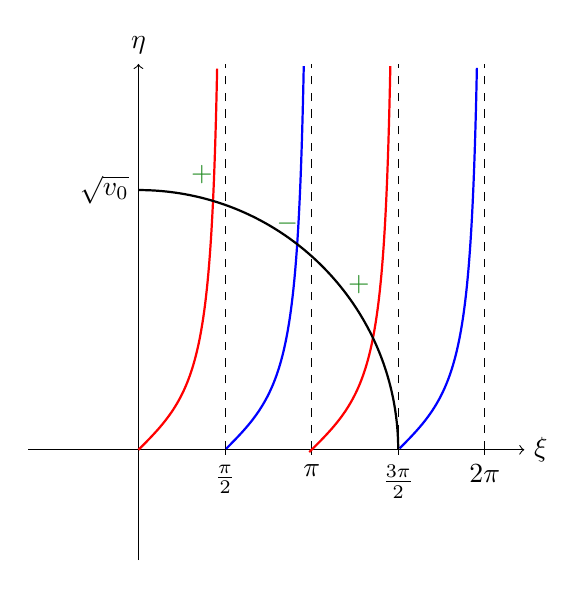
\begin{tikzpicture}[scale=0.7]
    % Assi
    \draw[->] (-2,0) -- (7,0) node[right] {$\xi$};
    \draw[->] (0,-2) -- (0,7) node[above] {$\eta$};
    
  % Etichette punti notevoli
    \draw (6.283,0.1) -- (6.283,-0.1) node[below] {$2\pi$};
    \draw (3.142,0.1) -- (3.142,-0.1) node[below] {$\pi$};
    \draw (1.571,0.1) -- (1.571,-0.1) node[below] {$\frac{\pi}{2}$};
    \draw (4.712,0.1) -- (4.712,-0.1) node[below] {$\frac{3\pi}{2}$};

    % Asintoti verticali tratteggiati
    \draw[dashed] (1.571,0) -- (1.571,7);
    \draw[dashed] (4.712,0) -- (4.712,7);
     \draw[dashed] (3.142,0) -- (3.142,7); 
     \draw[dashed] (6.283, 0) -- (6.283, 7);

    % Primo ramo positivo da 0 a poco prima di π/2
    \draw[thick, red, domain=0:1.43, smooth, samples=200] 
        plot (\x,{tan(\x r)});

    % Secondo ramo positivo da π a poco prima di 3π/2
    \draw[thick, red, domain=3.1:4.57, smooth, samples=200] 
        plot (\x,{tan(\x r)});

    % Terzo ramo (blu) positivo da poco dopo π/2 a poco prima di π
    \draw[thick, blue, domain=1.59:3, smooth, samples=200] 
        plot (\x,{-cot(\x r)});

    % Quarto ramo positivo da poco dopo 3π/2 a poco prima di 2π
    \draw[thick, blue, domain=4.74:6.14, smooth, samples=200] 
        plot (\x,{-cot(\x r)});
        
        % Semicirconferenza nel secondo quadrante, raggio 3/2 pi, centro (0,0)
    \draw[thick] (4.7124,0) arc[start angle=0, end angle=90, radius=4.7124];
    
    %%%
    \node[left] at (0, 4.7124) {$\sqrt{v_0}$};
    
    %%%
     \node[ForestGreen] at (2.7, 4.1) {$-$};
     \node[ForestGreen] at (1.15, 5) {$+$};
     \node[ForestGreen] at (4, 3) {$+$};

\end{tikzpicture}
\end{minipage}
\hfill
\begin{minipage}{0.5\textwidth}

	Nel grafico, le linee rosse sono le funzioni $\textcolor{red}{\eta = \xi \, \tan\xi}$ e le linee blu sono le funzioni $\textcolor{blue}{\eta = - \xi \, \cot\xi}$. Le ascisse $\xi$ dei punti di intersezione fra queste curve e la circonferenza nel primo quadrante (in cui $\tilde{k}, |k| > 0$ e quindi $\xi, \eta > 0$) danno i valori di $k$ tali per cui ho soluzioni pari (in rosso) e/o soluzioni disparti (in blu). Al variare del raggio $\sqrt{v_0}$ hp un certo numero di soluzioni pari e dispari. In generale:
	
\begin{align*}
	\qty(n-1)\,\pi < \sqrt{v_0} < n\pi 
\end{align*}

	con $n$ stati pari ed $n$ stati dispari ($n^+, n^-$).
	
\end{minipage}
%%%%%%%
\vspace{1em}
%%%%%%%
	
	Quali sono le energie ammesse in questo potenziale?
	\\
	\\
	A seconda del variare di $\xi$ si hanno diversi valori energetici possibili. Ad esempio, sia $\xi \leq \pi/2$: dal grafico osserviamo che esiste un'unica soluzione a parità positiva. Esplicitando la condizione si ha:
	
\begin{align*}
	\xi \leq \pi/2 \, \Rightarrow \, \frac{\tilde{k}a}{2} \leq \frac{\pi}{2} \, \Rightarrow \, \frac{2m}{\hbar^2} \, \qty(E + V_0) \, a^2 \leq \pi^2
\end{align*}

	ossia:
	
\begin{align*}
	E \leq \frac{\hbar^2 \, \pi^2}{2ma^2} - V_0 \, \equiv \, V_1 - V_0
\end{align*}

	In maniera analoga se consideriamo l'intervallo successivo, ho due soluzioni a parità definita, con energia:
	
\begin{align*}
	V_1 - V_0 \leq E \leq 4V_1 - V_0
\end{align*}

	allora iterando il ragionamento, nell'approssimazione in cui $V_0 >> V_1$, per i livelli energetici più bassi si ha:
	
\begin{align*}
	E \simeq \frac{n^2 \hbar^2 \pi^2}{2ma^2} - V_0
\end{align*}

	Cosa succede allora nel limite $\sqrt{v_0} \to \infty$? 
	\\
	\\
	In questo caso ho che $V_0 \to \infty$, cioè sono nel caso di \textbf{buca infinita di potenziale}. In questa situazione, la funzione d'onda assume una forma analitica piuttosto semplice, ovvero:

\begin{align*}
	\psi_n(x) = \sqrt{\frac{2}{a}} \sin\qty(\frac{n\pi}{a} \, x)
\end{align*}

	e allora le energie permesse sono:
	
\begin{align*}
	E_n = \frac{\hbar^2k^2}{2m} = \frac{n^2 \hbar^2 \pi^2}{2ma^2}
\end{align*}

\begin{myapprf}
	Facciamo ora un \textit{approfondimento}, piuttosto importante che introduce un teorema famoso. 
	\\
	\\
	In un potenziale simmetrico $V(x)$ gli stati legati hanno parità definita alterna e lo stato ad energia più bassa ha sempre parità $+1$ (vero solo in una dimensione). Ciò deriva dal teorema spettrale. Introduciamo allora il \textbf{teorema dei nodi}:
	\\
	\\
	\textit{Si consideri un sistema con un solo grado di libertà e siano: $E_0 < E_1 < \ldots < E_n$ gli autovalori discreti della Hamiltoniana ordinati in senso crescente e $\psi_0(x), \ldots, \psi_n(x)$ le corrispondenti autofunzioni. Allora indipendentemente dalla parità, l'$n$-esimo livello $E_n$ di autofunzione $\psi_n(x)$ ha $n$ nodi.} 
	
%%%%%%%
\vspace{1em}
%%%%%%%
\begin{center}
\begin{tikzpicture}[scale=0.7]
    % Assi
    \draw[->] (-5,0) -- (5,0) node[right] {$x$};
    \draw[->] (0,-5) -- (0,5) node[above] {$\psi_E(x)$};

    % eq 1
    \draw[thick, red, domain=-3.14:3.14, smooth, samples=200] 
        plot (\x,{-2*sin(\x r)});

    % eq 2
    \draw[thick, blue, domain=-3.14:3.14, samples=200, smooth] 
         plot (\x,{25*exp(-(\x)^2)/(2*1.9^2)});
      
    %%%
     \node[red] at (-2.7, 2.5) {$-$};
     \node[blue] at (1.15, 3.8) {$+$};

\end{tikzpicture}
\end{center}
\end{myapprf}

\subsection{Barriera di Potenziale Finita}

	Si consideri una \textbf{barriera di potenziale}, ossia un potenziale del seguente tipo:
	
\begin{empheq}[left={V(x) = \empheqlbrace}]{align*}
	& 0 \quad \text{se} \quad |x| > a \\
	& V_0 \quad \text{se} \quad |x| < a 
\end{empheq}

%%%%%%%
\vspace{1em}
%%%%%%%
\begin{minipage}{0.65\textwidth}
\begin{tikzpicture}[scale=0.8]
	% Assi
    	\draw[->] (-5, 0) -- (5, 0) node[right] {$x$};
    	\draw[->] (0, -1) -- (0, 5) node[above] {$V(x)$};
	
	% funzione
	\draw[thick, red] (-3, 0) -- (-3, 3.5);
	\draw[thick, red] (-3, 3.5) -- (3, 3.5);
	\draw[thick, red] (3, 3.5) -- (3, 0);
	
	% scritte
	\node[red] at (3, 4) {$V_0$};
	\node[below] at (-3, 0) {$-a$};
	\node[below] at (3, 0) {$+a$};
	
\end{tikzpicture}
\end{minipage}
\hfill
\begin{minipage}{0.38\textwidth}
	riprendiamo inoltre l'equazione di Schrodinger unidimensionale. Essa è:
\begin{enumerate}
	\item Lineare omogenea.
	\item A coefficienti reali e a valori complessi: se $\psi_E(x)$ è soluzione allora $\psi_E^*(x)$ lo è anche.
	\item È priva del termine $\psi_E'(x)$.
\end{enumerate}
\end{minipage}
%%%%%%%
\vspace{1em}
%%%%%%%

	Dunque se $\dim\mathcal{H}_E = 1$, la funzione d'onda di uno stato legato è "quasi" reale a meno di un numero:

\begin{align*}
	\psi_E^*(x) = \lambda \, \psi_E(x) \, \Rightarrow \, \psi_E(x) = \lambda^* \, \psi_E^*(x) = \lambda^* \, \lambda \psi_E(x) = |\lambda^2| \, \psi_E(x) \, \Rightarrow \, |\lambda^2| = 1 
\end{align*}

	pertanto deve valere che $\lambda$ è una fase del tipo:
	
\begin{align*}
	\lambda = e^{ \, i\alpha}
\end{align*}

	e dunque possiamo scrivere:
	
\begin{align*}
	\psi^* = e^{ \, i\alpha} \, \psi \, \Rightarrow \, e^{\, -i \alpha/2 } \psi^* = e^{\, i \alpha/2 } \psi \, \Rightarrow \, \qty(e^{\, i \alpha/2 } \psi)^* = e^{\, i \alpha/2 }\psi
\end{align*}

	Ridefinendo:
	
\begin{align*}
	\tilde{\psi}(x) = e^{\, i \alpha/2} \psi(x)
\end{align*}

	allora ho che:
	
\begin{align*}
	\tilde{\psi}^* = \tilde{\psi}
\end{align*}

	e quindi deve valere che $\psi(x)$ è reale. Essa sarà del tipo:

\begin{empheq}[left={\psi_E(x)=\empheqlbrace}]{align*}
	& Ae^{\, ikx} + Be^{\, -ikx} \qquad \text{se} \quad x \to -\infty \\
  	& \psi_E(x) \qquad \text{se} \quad -\infty < x < +\infty \\
	& Ce^{\, ikx} + De^{\, -ikx} \qquad \text{se} \quad x \to +\infty
\end{empheq}

	ossia, considerando $0 < E < V_0$, classicamente, se si invia ad esempio da $x < 0$ una particella contro la barriera, essa viene riflessa e torna indietro. Secondo la meccanica quantistica invece, si ha una probabilità non nulla che la particella attraversi la barriera di potenziale, questo fenomeno si chiama: \textbf{effetto tunnel}.
	\\
	\\
	Tornando a prima analogamente alla buca di potenziale, i coefficienti sono legati tra loro dalla \textit{matrice di trasmissione:}
	
\begin{align*}
	\mqty(C \\ D) = \mathcal{T} \, \mqty(A \\ B) = \mqty( \alpha & \beta \\ \gamma & \delta) \mqty(A \\ B)
\end{align*}

	Che proprietà ha $\mathcal{T}$ in questo caso? Ho che:
	
\begin{empheq}[left={\psi_E^*(x)=\empheqlbrace}]{align*}
	& B^* \, e^{\, ikx} + A^* \, e^{\, -ikx} \qquad \text{se} \quad x \to -\infty \\
  	& D^* \, e^{\, ikx} + C^* \, e^{\, -ikx} \qquad \text{se} \quad x \to +\infty 
\end{empheq}

	Ma, poiché $\psi_E^*$ è soluzione dello stesso problema, ho allora che:
	
\begin{align*}
	\mqty(D^* \\ C^*) =  \mqty( \alpha & \beta \\ \gamma & \delta) \mqty(B^* \\ A^*)
\end{align*}

	da cui:

\begin{align*}
	\mqty(D \\ C) =  \mqty( \alpha^* & \beta^* \\ \gamma^* & \delta^*) \mqty(B \\ A)
\end{align*}

	quindi:

\begin{empheq}{align*}
	& C = \alpha A + \beta B \quad , \quad C = \gamma^* B + \delta^* A \\
	&D = \gamma A + \delta B \quad , \quad D = \alpha^* B + \beta^* A
\end{empheq}

	Da cui, per confronto, ho $\alpha = \delta^*$ e $\beta = \gamma^*$ e quindi:

\begin{align*}
	\mathcal{T} = \mqty(\alpha & \beta \\ \beta^* & \alpha^*)
\end{align*}	

	Che condizioni ho sulla matrice $\mathcal{T}$?
	\\
	\\
	Per un potenziale simmetrico e costante nel tempo la dinamica quantistica è invariante rispetto all'inversione temporale. Poiché si ha invarianza per inversione temporale, la funzione d'onda invertita temporalmente avrà direzione di propagazione inversa a quella iniziale. Ciò significa cambiare il segno alle fasi ($x \to - x$), ossia coniugare la funzione d'onda iniziale e quindi la matrice di trasmissione che descrive la relazione tra le ampiezze. L'invarianza per inversione temporale inoltre ci permette di dire che la matrice di trasmissione nella direzione opposta sarà la matrice inversa di quella originale, perciò possiamo concludere che:
	
\begin{align*}
	\mathcal{T}^{\, -1} = \mathcal{T}^*
\end{align*}

	In questo modo si ottiene:
	
\begin{align*}
	\mqty(\alpha^* & - \beta \\ - \beta^* & \alpha) = \mqty(\alpha^* & \beta^* \\ \beta & \alpha)
\end{align*}

	da cui, per confronto degli elementi, si ha l'equazione:
	
\begin{align*}
	-\beta = \beta^*
\end{align*}
	
	In particolare, scrivendo $\beta = a + i b$, otteniamo che dall'imporre $\beta = - \beta^*$ seguono $a = 0$ e $\beta = ib$, con $b \in \mathbb{R}$. Ne concludiamo che $\beta$ è un immaginario puro.
	\\
	\\
	Osserviamo che ora se $\psi_E\qty(x)$ è soluzione, allora la funzione:

\begin{nb}
\begin{align*}
	W\qty(x) = \psi_E^*\qty(x) \, \psi_E'\qty(x) - \qty[\psi_E^*\qty(x)]' \psi_E\qty(x)
\end{align*}

	detta \textbf{Wronskiano}, è costante.
\end{nb}

	Infatti:
	
\begin{align*}
	W'\qty(x) & = \qty[ \psi_E^*\qty(x)]' \psi_E'\qty(x) + \psi_E^*\qty(x)\psi_E''\qty(x) - \qty[\psi_E^*\qty(x)]'' \psi_E\qty(x) - \qty[\psi_E^*\qty(x)]' \psi_E'\qty(x) \\
	& = \psi_E^*\qty(x) \frac{2m}{\hbar^2} \qty[V\qty(x) - E ] \psi_E\qty(x) - \frac{2m}{\hbar^2} \qty[V\qty(x) - E] \psi_E^*\qty(x) \psi_E\qty(x) \\
	& = 0
\end{align*}

	Si applica ora questo risultato alla soluzione dell'equazione di Schrodinger per una barriera di potenziale $V\qty(x)$ che tende a zero per $x \to \pm \infty$. Essa ha la forma:

\begin{empheq}[left={\psi_E\qty(x)=\empheqlbrace}]{align*}
	& A e^{\, ikx} + B e^{\, -ikx} \qquad \text{se} \quad x \to -\infty \\
  	& C e^{\, ikx} + D e^{\, -ikx} \qquad \text{se} \quad x \to +\infty 
\end{empheq}

	con $k^2 = 2mE / \hbar^2$. Dove il $V\qty(x)$ è quindi:

%%%%%%%
\vspace{1em}
%%%%%%%
\begin{center}
\begin{tikzpicture}[scale=0.7]
    % Assi
    \draw[->] (-5,0) -- (5,0) node[right] {$x$};
    \draw[->] (0,-1) -- (0,5) node[above] {$V\qty(x)$};

    % eq 2
    \draw[thick, blue, domain=-3.14:3.14, samples=200, smooth] 
         plot (\x,{38*exp(-(\x)^2)/(2.3*1.9^2)});

\end{tikzpicture}
\end{center}
%%%%%%%
\vspace{1em}
%%%%%%%

\begin{empheq}{align*}
	& \lim_{x \to - \infty} W\qty(x) \equiv W\qty(- \infty) = 2ik \, \qty(\qty|A|^2 - \qty|B|^2) \\
  	& \lim_{x \to + \infty} W\qty(x) \equiv W\qty( + \infty) = 2ik \, \qty(\qty|C|^2 - \qty|D|^2)
\end{empheq}

	da cui ho:
	
\begin{align*}
	\qty|A|^2 - \qty|B|^2 = \qty|C|^2 - \qty|D|^2
\end{align*}

	ma per quanto detto prima, $C$ e $D$ sono funzioni lineari di $A$ e $B$:
	
\begin{align*}
	\qty|A|^2 - \qty|B|^2 = \qty|\alpha A + \beta B|^2 - \qty|\beta^* A + \alpha^* B|^2 = \qty(\qty|\alpha|^2 - \qty|\beta|^2) \qty|A|^2 + \qty(\qty|\beta|^2 - \qty|\alpha|^2) \qty|B|^2
\end{align*}

	pertanto:
	
\begin{align*}
	\qty|\alpha|^2 - \qty|\beta|^2 = 1
\end{align*}

	se vogliamo riprodurre la situazione di una particella che arriva da sinistra (e che eventualmente può attraversare la barriera) cerchiamo soluzione che abbiano $A \neq 0$ e $D = 0$ (nessuna particella arriva da destra). Senza perdere di generalità poniamo quindi $A = 1$ e la soluzione diventa:

\begin{empheq}[left={\psi_E^+\qty(x)=\empheqlbrace}]{align*}
	& e^{\, ikx} + B e^{\, -ikx} \qquad \text{se} \quad x \to -\infty \\
  	& C e^{\, ikx} \qquad \text{se} \quad x \to +\infty 
\end{empheq}

	posso scrivere $B$ e $C$ in termini di $\alpha$ e di $\beta$:

\begin{empheq}[left=\empheqlbrace]{align*}
	& C = \alpha + \beta B \\
  	& 0 = \beta^* + \alpha^* B
\end{empheq}

	quindi:

\begin{empheq}[left=\empheqlbrace]{align*}
	& B = - \frac{\beta^*}{\alpha^*} \\
  	& C = \frac{1}{\alpha^*}
\end{empheq}

	La soluzione $\psi_E^+\qty(x)$ può essere interpretata  come un flusso di particelle di impulso $k$ provenienti da $x \to - \infty$, una parte delle quali, proporzionale a $\qty|B|^2$ è riflessa dalla barriera, e una parte, proporzionale a $\qty|C|^2$ è trasmessa dalla barriera verso $x \to + \infty$. 
	\\
	\\
	Definiamo pertanto i coefficienti di \textbf{riflessione}, $R$, e di \textbf{trasmissione}, $T$, come:
	
\begin{align*}
	R = \qty|-\frac{\beta^*}{\alpha^*}|^2 = \qty|\frac{\beta}{\alpha}|^2 \quad , \quad T = \qty|\frac{1}{\alpha^*}|^2 = \frac{1}{\qty|\alpha|^2}
\end{align*}

	si noti che:
	
\begin{align*}
	R + T = \frac{\qty|\beta|^2 + 1}{\qty|\alpha|^2} = 1
\end{align*}

\subsection{Buca di potenziale a $\delta\qty(x)$:}

	Si consideri un potenziale nella forma:
	
\begin{align*}
	V\qty(x) = - \alpha \, \delta\qty(x)
\end{align*}

	dove $\alpha$ è una costante positiva arbitraria. La funzione delta ha le dimensioni dell'inverso di una lunghezza, quindi $\alpha$ ha le dimensioni di un'energia per una lunghezza. L'equazione di Schrodinger per tale potenziale prende la forma:
	
\begin{align*}
	- \frac{\hbar^2}{2m} \psi'' - \alpha \, \delta\qty(x) \, \psi = E \psi
\end{align*}

	consideriamo separatamente gli stati legati ($E < 0$) e gli stati diffusi ($E > 0$).
	
\begin{itemize}
	\item \textbf{Stati legati:} $E < 0$
	
		Iniziando dagli stati legati, nella regione $x < 0$ si ha $V\qty(x) = 0$, pertanto:
		
	\begin{align*}
		\psi'' = - \frac{2mE}{\hbar^2} \psi \equiv \kappa^2 \psi
	\end{align*}
	
		con:
		
	\begin{align*}
		\kappa = \frac{\sqrt{-2mE}}{\hbar}
	\end{align*}
	
		in cui, poiché $E < 0$ per ipotesi, $\kappa$ è positivo e reale. La soluzione generale dell'equazione è:
		
	\begin{align*}
		\psi^-\qty(x) = A e^{- \kappa x} + B e^{\kappa x}
	\end{align*}
	
		ma, poiché il primo termine esplode per $x \to - \infty$, scegliamo $A	 = 0$:
		
	\begin{align*}
		\psi^-\qty(x) = B e^{\kappa x} \quad \text{con} \quad x < 0
	\end{align*}

		Nella regione $x > 0$ il potenziale è di nuovo nullo e la soluzione generale è nella forma:
		
	\begin{align*}
		\psi^+\qty(x) = F e^{-\kappa x} + G e^{\kappa x} 
	\end{align*}
		
		e questa volta il secondo termine esplode per $x \to + \infty$, da cui $G = 0$:
		
	\begin{align*}
		\psi^+\qty(x) = F e^{-\kappa x} \quad \text{con} \quad x > 0
	\end{align*}
	
		Rimane dunque solo da unire le due funzioni assieme, usando condizioni al contorno appropriate in $x = 0$. Le condizioni al contorno in genere richiedono che la funzione sia sempre continua e che la sua derivata prima sia continua eccetto che nei punti in cui il potenziale diverge. La prima richiesta, in questo caso, ci dice che $F = B$, cioè:
	
	\begin{empheq}[left={\psi \qty(x)=\empheqlbrace}]{align*}
		& B e^{\kappa x} \quad \text{con} \quad x \leq 0 \\
  		& B e^{-\kappa x} \quad \text{con} \quad x \geq 0
	\end{empheq}
	
		mentre la seconda richiesta non ci dice nulla di che: è il caso eccezionale in cui $V$ è infinito nel punto di raccordo tra le funzioni, ed è chiaro che la funzione è patologica in $x = 0$. Evidentemente la funzione delta determina la discontinuità nella derivata prima di $\psi$ in $x = 0$. Come si aggira il problema?
		\\
		\\
		L'idea è quella di integrare l'equazione tra $- \varepsilon$ e $+ \varepsilon$ e prende successivamente il limite $\varepsilon \to 0$:
		
	\begin{align*}
		-\frac{\hbar^2}{2m} \int_{- \varepsilon}^{+ \varepsilon} \psi'' \dd x + \int_{- \varepsilon}^{+ \varepsilon} V\qty(x) \psi\qty(x) \, \dd x = E \int_{- \varepsilon}^{+ \varepsilon} \psi\qty(x) \, \dd x
	\end{align*}
	
		Il primo integrale restituisce semplicemente la derivata prima valutata in due punti, l'ultimo integrale è invece nullo nel limite di $\varepsilon \to 0$, poiché è l'area di un punto di larghezza tendente a zero e altezza finita. Pertanto:

	\begin{align*}
		\Delta \psi'\qty(x) \equiv \psi'\qty(+ \varepsilon) - \psi'\qty(-\varepsilon) = \frac{2m}{\hbar^2} \lim_{\varepsilon \to 0} \int_{- \varepsilon}^{+ \varepsilon} V\qty(x) \psi\qty(x) \, \dd x
	\end{align*}	
	
		In generale il limite del membro di destra è nullo ed in ciò risiede il motivo per cui la derivata prima è ordinariamente continua. Tuttavia, quando $V\qty(x)$ è infinito sul contorno, questo procedimento fallisce. In particolare, per il nostro potenziale:
		
	\begin{align*}
		V\qty(x)= - \alpha \delta\qty(x)
	\end{align*}
	
		la proprietà della funzione delta ci da:
		
	\begin{align*}
		\Delta \psi'\qty(x) = - \frac{2m\alpha}{\hbar^2} \psi\qty(0)
	\end{align*}
	
		da cui:
		
	\begin{empheq}{align*}
		& \Delta \psi'\qty(x) = - 2 B \frac{m \alpha}{\hbar^2} \\
  		& \Delta \psi'\qty(x) = - 2 B \kappa
	\end{empheq}
	
		allora:
	
	\begin{align*}
		\kappa = \frac{m \alpha}{\hbar^2}
	\end{align*}

		e l'energia ammessa è:
		
	\begin{align*}
		E = - \frac{\hbar^2 \kappa^2}{2m} = - \frac{m \alpha^2}{2 \hbar^2}
	\end{align*}

		infine normalizziamo $\psi$:
		
	\begin{align*}
		\int_{- \infty}^{+ \infty} \qty|\psi\qty(x)|^2 \, \dd x = 2 \, \qty|B|^2 \int_0^{+ \infty} e^{-2 \kappa x} \dd x = \frac{\qty|B|^2}{\kappa} = 1
	\end{align*}
	
		da cui, scegliendo per comodità la soluzione positiva:
		
	\begin{align*}
		B = \sqrt{\kappa} = \frac{\sqrt{m \alpha}}{\hbar}
	\end{align*}
	
		Risulta evidente che la buca di potenziale a delta, indipendentemente dalla sua "intensità" $\alpha$, ha esattamente uno stato legato:
	
	\begin{nb}
	\begin{align*}
		\psi\qty(x) = \frac{\sqrt{m \alpha}}{\hbar} \, e^{\frac{- m \alpha \qty|x|}{\hbar^2}}
	\end{align*}
	\end{nb}
	
	%%%%%%%
	\vspace{1em}
	%%%%%%%	
	\begin{tikzpicture}
    \begin{axis}[
        axis lines = middle,
        axis line style = {-}, % Removes the arrows from the axes
        xlabel = {$x$},
        ylabel = {$\psi(x)$},
        x label style = {anchor=north},
        y label style = {anchor=west},
        xmin = -4.5, xmax = 4.5,
        ymin = -0.1, ymax = 1.3,
        xtick = \empty,
        ytick = \empty, % Removes the default bar/tick mark
        samples = 150,
        width = 12cm,
        height = 7cm,
        clip = false
    ]
    
    % The wavefunction curve (now red)
    \addplot[thick, red, domain=-4.2:4.2] {exp(-abs(x))};
    
   % The label only (no line, text is red)
    \node[red, right] at (2.2, 0.6) {$\sqrt{\kappa} e^{-\kappa x}$};
                 
    % The thick black dot at the peak with its label
    \filldraw[black] (0, 1) circle (2pt) node[right=4pt] {$\sqrt{\kappa}$};
                 
    \end{axis}
\end{tikzpicture}
	%%%%%%%
	\vspace{1em}
	%%%%%%%

	\item \textbf{Stati diffusi:} $E > 0$
	
		Per quanto riguarda gli stati diffusi, quelli con $E > 0$, nella regione $x < 0$ si ha:
		
	\begin{align*}
		\psi'' = - \frac{2mE}{\hbar^2} \psi \equiv - k^2 \psi
	\end{align*}
	
		dove:
		
	\begin{align*}	
		k \equiv \frac{\sqrt{2mE}}{\hbar}
	\end{align*}
	
		è reale e positivo. La soluzione generale è:
		
	\begin{align*}
		\psi^-\qty(x) = A e^{\, i k x} + B e^{ \, - i k x}
	\end{align*}
	
		e in questo caso non possiamo dire nulla sulle singole ampiezze, dal momento che nessuna di esse diverge. Analogamente, per $x > 0$:
		
	\begin{align*}
		\psi^+\qty(x) = F e^{\, i k x} + G e^{ \, - i k x}
	\end{align*}

		La continuità di $\psi\qty(x)$ in $x = 0$ richiede che:
		
	\begin{align*}
		F + G = A + B
	\end{align*}

		e le derivate prime sono:
		
	\begin{empheq}[left=\empheqlbrace]{align*}
		& \dv{\psi^+}{x} = i k \, \qty(F e^{\, i k x} + G e^{ \, - i k x}) \\
  		& \dv{\psi^-}{x} = i k \, \qty(A e^{\, i k x} - B e^{ \, - i k x})
	\end{empheq}
		
		e quindi:
		
	\begin{empheq}[left=\empheqlbrace]{align*}
		& \dv{\psi}{x} \big |_+ = i k \, \qty(F + G ) \\
  		& \dv{\psi}{x} \big |_- = i k \, \qty(A - )
	\end{empheq}
	
		allora:
		
	\begin{align*}
		\Delta \psi' \qty(x) = i k \, \qty( F - G - A + B)
	\end{align*}	
	
		contemporaneamente $\psi\qty(0) = A + B$, pertanto la seconda condizione al contorno ci dice che:
		
	\begin{align*}
		 i k \, \qty( F - G - A + B) = -\frac{2 m \alpha}{\hbar^2} \, \qty(A + B)
	\end{align*}
	
		oppure in maniera più compatta:
		
	\begin{align*}
		F - G = A \, \qty( 1+ 2 i\beta) - B\, \qty(1 - 2 i\beta)
	\end{align*}
		
		con $\beta \equiv \frac{m \alpha}{\hbar^2 k}$.
		\\
		\\
		Imposte entrambe le condizioni al contorno, rimaniamo con due equazioni in quattro incognite ($A, B, F, G$), o 5 se includiamo $k$. La normalizzazione non aiuta, poiché non abbiamo uno stato normalizzabile. Poiché vale che $e^{\, ikx}$ dà origine (quando accoppiato con il fattore dipendente dal tempo $e^{\, - iEt/\hbar}$) ad una funzione d'onda che si propaga verso destra, mentre $e^{\,- ikx}$ dà luogo ad una funzione d'onda che si propaga verso sinistra, l'ampiezza $A$ è l'ampiezza di un'onda che arriva da sinistra, mentre l'ampiezza $B$ è l'ampiezza di un'onda che torna verso sinistra. Analogamente l'ampiezza $F$ è l'ampiezza di un'onda che si propaga verso destra, e l'ampiezza $G$ è l'ampiezza di un'onda che arriva da destra.

	%%%%%%%
	\vspace{1em}
	%%%%%%%
	\begin{tikzpicture}
    \begin{axis}[
        axis lines = middle,
        axis line style = {->},
        xlabel = {$x$},
        x label style = {anchor=north west},
        xmin = -5, xmax = 5,
        ymin = -4.5, ymax = 3,
        xtick = \empty,
        ytick = \empty,
        width = 15cm,
        height = 9cm,
        clip = false
    ]
    
    % The Dirac delta potential well (represented by a very narrow, deep Gaussian)
    % We use 200 samples so the sharp point renders smoothly
    \addplot[thick, black, domain=-4.8:4.8, samples=200] {-4*exp(-100*x^2)};
    
    % --- LEFT SIDE WAVES (x < 0) ---
    
    % Incident wave (A) - Arrow pointing right
    \draw[-stealth] (-3.5, 1.5) -- (-1.5, 1.5) node[midway, above] {$A e^{ikx}$};
    
    % Reflected wave (B) - Arrow pointing left
    \draw[-stealth] (-1.5, 0.5) -- (-3.5, 0.5) node[midway, below] {$B e^{-ikx}$};
    
    % --- RIGHT SIDE WAVES (x > 0) ---
    
    % Transmitted wave (F) - Arrow pointing right
    \draw[-stealth] (1.5, 1.5) -- (3.5, 1.5) node[midway, above] {$F e^{ikx}$};
    
    % Incident wave from the right (G) - Arrow pointing left
    \draw[-stealth] (3.5, 0.5) -- (1.5, 0.5) node[midway, below] {$G e^{-ikx}$};

    \end{axis}
\end{tikzpicture}
	%%%%%%%
	\vspace{1em}
	%%%%%%%
		
		In un tipico esperimento di scattering, le particelle vengono lanciate da una direzione, ad esempio, da sinistra. In tal caso, l'ampiezza dell'onda che arriva da destra sarà nulla:
		
	\begin{align*}
		G = 0
	\end{align*}
	
		Il fattore $A$ è l'ampiezza dell'onda incidente, mentre il fattore $B$ dell'onda riflessa. Il fattore $F$ assume invece il significato ampiezza dell'onda trasmessa. Risolvendo le equazioni per $B$ e per $F$ si trova:
		
	\begin{align*}
		\mqty(B \\ F) = \mqty(\frac{i \beta}{1 - i \beta } \\ \frac{1}{1 - i \beta }) \, A
	\end{align*}
		
		Se avessimo scelto l'onda incidente da destra, in modo analogo si pone $A = 0$ e quindi $G$ è l'ampiezza incidente, $F$ è l'ampiezza riflessa e $B$ l'ampiezza trasmessa.
		
\end{itemize}

\section{Sistemi unidimensionali nel formalismo dei coefficienti $R$ e $T$:}

	Adesso che abbiamo introdotto i coefficienti di riflessione $R$ e di trasmissione $T$, vediamo brevemente come vengono applicati nello studio dei sistemi presi in esame.
	
\subsection{Gradi di potenziale} 
	
	Nel caso del gradino di potenziale distinguiamo nei due casi:
	
\begin{itemize}
	\item \textbf{Riflessione parziale:} $E > V_0$
	
		Poniamo
		
	\begin{align*}
		k_1 \equiv \sqrt{\frac{2mE}{\hbar^2}} \quad , \quad k_2 \equiv \sqrt{\frac{2m\qty(E-V_0)}{\hbar^2}}
	\end{align*}
		
		e la soluzione, come già detto, assume la forma:
		
	\begin{empheq}[left={\psi_E \qty(x)=\empheqlbrace}]{align*}
		& A e^{ \, i k x} + B e^{ \, - i k x} \quad \text{se} \quad x < 0 \\
  		& A' e^{ \, i k' x} + B' e^{ \, - i k' x} \quad \text{se} \quad x > 0
	\end{empheq}
	
		da cui, imponendo la continuità $\psi_E\qty(x)$ e della sua derivata prima in $x = 0$, scegliamo $B' = 0$ (sottintendendo quindi che siamo nel caso di una particella che arriva da $x = - \infty$) e tale scelta ci permette di scrivere:
		
	\begin{align*}
		\frac{B}{A} = \frac{k_1 - k_2}{k_1 + k_2} \quad , \quad \frac{A'}{A} = \frac{2 k_1}{k_1 + k_2}
	\end{align*}
		
		da cui, senza darne una dimostrazione, si ha:
		
	\begin{align*}
		R = \qty|\frac{B}{A}|^2 = 1 - \frac{4 k_1 k_2}{\qty(k_1 + k_2)^2} \quad , \quad T = \frac{k_2}{k_1} \, \qty|\frac{A'}{A}|^2 = \frac{4 k_1 k_2}{\qty(k_1 + k_2)^2}
	\end{align*}

	\item \textbf{Riflessione totale:} $0 < E < V_0$
		
		In questo caso definiamo:
		
	\begin{align*}
		\rho_2 = \sqrt{\frac{2m \qty(V_0 - E)}{\hbar^2}}
	\end{align*}
	
		in modo tale che la soluzione assuma la forma:
		
	\begin{empheq}[left={\psi_E \qty(x)=\empheqlbrace}]{align*}
		& A e^{ \, i k x} + B e^{ \, - i k x} \quad \text{se} \quad x < 0 \\
  		& A' e^{ \, \rho_2 x} + B' e^{ \, \rho_2 x} \quad \text{se} \quad x > 0
	\end{empheq}
	
		affinché la soluzione per $x \to + \infty$ si deve imporre $A' = 0$ e le richieste di continuità e derivabilità in $x = 0$ portano a scrivere:
		
	\begin{align*}
		\frac{B}{A} = \frac{k_1 - i \rho_2}{k_1 + i \rho_2} \quad , \quad \frac{B'}{A} = \frac{2k_1}{k_1 + i \rho_2} 
	\end{align*}

		da cui si evince subito che:
		
	\begin{align*}
		R = \qty|\frac{k_1 - i\rho_2}{k_1 + i\rho_2}| = 1
	\end{align*}
	
		confermando la riflessione totale della particella, diventando coerente con il comportamento classico.
		
\end{itemize}
	
	
\subsection{Barriera di potenziale finita}

	Considerando una barriera di potenziale di altezza $V_0$ e larghezza $a$, centrata in $x_0 = \frac{a}{2}$:
	
\begin{empheq}[left={V\qty(x)=\empheqlbrace}]{align*}
	& V_0 \quad \text{se} \quad  0 < x < a \\
  	& 0 \qquad \text{altrimenti}
\end{empheq}

	Distinguiamo ora in due casi, dove esporremo i risultati, senza darne dimostrazione:
	
\begin{itemize}
	\item \textbf{Risonanza:} $E > V_0$
	
		In questo caso la soluzione sarà del tipo:
	
	\begin{empheq}[left={\psi_E\qty(x)=\empheqlbrace}]{align*}
		& A_1 e^{ik_1x} + A_1' e^{- ik_1x} \quad \text{se} \quad x < a \\
		& A_2 e^{ik_2x} + A_2' e^{- ik_2x} \quad \text{se} \quad  0 < x < a \\
  		& A_3 e^{ik_1x} + A_3' e^{- ik_1x} \quad \text{se} \quad x > a
	\end{empheq}
	
		in cui scegliamo $A_3' = 0$ (particella proveniente da $x = - \infty$). Le condizioni di continuità e derivabilità in $x = a$ permettono di scrivere $A_2$ e $A_2'$ in termini $A_3$, e quelle in $x = 0$ permettono di scrivere $A_1$ e $A_1'$ in termini di $A_2$ e $A_2'$ (e di conseguenza in termini di $A_3$). Si trova quindi che:
		
	\begin{align*}
		& R = \qty|\frac{A_1'}{A_1}|^2 = \frac{\qty(k_1^2 - k_2^2)^2 \sin^2\qty(k_2 a)}{4 k_1^2 k_2^2 + \qty(k_1^2 - k_2^2)^2 \sin^2\qty(k_2 a)} \\
		& T = \qty|\frac{A_3}{A_1}|^2 = \frac{ 4 k_1^2 k_2^2}{4 k_1^2 k_2^2 + \qty(k_1^2 - k_2^2)^2 \sin^2\qty(k_2 a)}
	\end{align*}
	
		da cui si vede facilmente che $R + T = 1$. Sostituendo le definizioni $k_1$ e $k_2$ si ottiene:
		
	\begin{align*}
		T = \frac{4 E \qty(E - V_0)}{4 E \qty(E - V_0) + V_0^2 \, \sin^2\qty[ \frac{\sqrt{2 m \qty(E - V_0)} \, a}{\hbar}]}
	\end{align*}	
	
		ossia la variazione del coefficiente di trasmissione $T$ rispetto alla larghezza della barriera $a$ è oscillante tra un valore minimo e $T = 1$: tale fenomeno è chiamato \textbf{risonanza di scattering}.
	
	\item \textbf{Effetto Tunnel:} $ 0 < E < V_0$
	
		Il procedimento da fare in questo caso è lo stesso fatto per l'esempio del gradino di potenziale: prendiamo il caso $E > V_0$ dalla barriera di potenziale e definiamo $\rho_2$ nello stesso modo e, successivamente, sostituiamo nelle equazioni $k_2$ con $- i \rho_2$. Ciò che si ottiene è:
		
	\begin{align*}
		T = \qty|\frac{A_3}{A_1}|^2= \frac{4 E \qty(E - V_0)}{4 E \qty(E - V_0) + V_0^2 \, \sin^2\qty[ \frac{\sqrt{2 m \qty(E - V_0)} \, a}{\hbar}]}
	\end{align*}
	
		con $R = 1 - T$. Quando $\rho_2 a >> 1$, si ha:
		
	\begin{align*}
		T \simeq \frac{16 E \, \qty(V_0 - E)}{V_0^2} \, e^{\, -2 \rho_2 a}
	\end{align*}
	
		Come già visto, contrariamente alle previsioni classiche, la particella ha una probabilità non nulla di attraversare la barriera di potenziale. La funzione d'onda nella regione classicamente proibita è non nulla, ma si comporta come un'onda evanescente con raggio di azione $1/\rho_2$. Quando $a < 1/\rho_2$, la particella ha una probabilità considerevole di attraversare la barriera tramite effetto tunnel.
		
\end{itemize}

\subsection{Buca di potenziale a $\delta\qty(x)$}

	Consideriamo il caso degli stati diffusi, nell'ipotesi dell'onda incidente proveniente da sinistra. Il coefficiente di riflessione in questo caso assume la forma:
	
\begin{align*}
	R \equiv \qty|\frac{B}{A}|^2 = \frac{\beta^2}{1 + \beta^2}
\end{align*}

	mentre il coefficiente di trasmissione è:
	
\begin{align*}
	T \equiv \qty|\frac{F}{A}|^2 = \frac{1}{1 + \beta^2}
\end{align*}

	in modo più completo, esplicitando $\beta$, si ha:
	
\begin{align*}
	& R = \frac{1}{1 + \frac{2 \hbar^2 E}{m \alpha^2}} \\
	& T = \frac{1}{1 + \frac{m \alpha^2}{2 \hbar^2 E}}
\end{align*}

	Maggiore è l'energia, maggiore è la probabilità di trasmissione.

